\documentclass[12pt,amstags,fleqn]{article}

% Uncomment only one of these lines:
\usepackage[mathlf,textlf,minionint]{MinionPro} \usepackage[T1]{fontenc} \usepackage{textcomp} \usepackage{amsthm}
%\usepackage{amssymb}

\usepackage{url}

\usepackage{xspace}

\usepackage{fancyvrb}
\usepackage{color}
\usepackage{fancyvrb}
\usepackage{color}

\newcommand\at{@}
\newcommand\lb{[}
\newcommand\rb{]}
\newcommand\PYbg[1]{\textcolor[rgb]{0.00,0.50,0.00}{\textbf{#1}}}
\newcommand\PYbf[1]{\textcolor[rgb]{0.73,0.40,0.53}{\textbf{#1}}}
\newcommand\PYbe[1]{\textcolor[rgb]{0.40,0.40,0.40}{#1}}
\newcommand\PYbd[1]{\textcolor[rgb]{0.73,0.13,0.13}{#1}}
\newcommand\PYbc[1]{\textcolor[rgb]{0.00,0.50,0.00}{\textbf{#1}}}
\newcommand\PYbb[1]{\textcolor[rgb]{0.40,0.40,0.40}{#1}}
\newcommand\PYba[1]{\textcolor[rgb]{0.00,0.00,0.50}{\textbf{#1}}}
\newcommand\PYaJ[1]{\textcolor[rgb]{0.73,0.13,0.13}{#1}}
\newcommand\PYaK[1]{\textcolor[rgb]{0.00,0.00,1.00}{#1}}
\newcommand\PYaH[1]{\fcolorbox[rgb]{1.00,0.00,0.00}{1,1,1}{#1}}
\newcommand\PYaI[1]{\textcolor[rgb]{0.69,0.00,0.25}{#1}}
\newcommand\PYaN[1]{\textcolor[rgb]{0.00,0.00,1.00}{\textbf{#1}}}
\newcommand\PYaO[1]{\textcolor[rgb]{0.00,0.00,0.50}{\textbf{#1}}}
\newcommand\PYaL[1]{\textcolor[rgb]{0.73,0.73,0.73}{#1}}
\newcommand\PYaM[1]{\textcolor[rgb]{0.74,0.48,0.00}{#1}}
\newcommand\PYaB[1]{\textcolor[rgb]{0.00,0.25,0.82}{#1}}
\newcommand\PYaC[1]{\textcolor[rgb]{0.67,0.13,1.00}{#1}}
\newcommand\PYaA[1]{\textcolor[rgb]{0.00,0.50,0.00}{#1}}
\newcommand\PYaF[1]{\textcolor[rgb]{1.00,0.00,0.00}{#1}}
\newcommand\PYaG[1]{\textcolor[rgb]{0.10,0.09,0.49}{#1}}
\newcommand\PYaD[1]{\textcolor[rgb]{0.25,0.50,0.50}{\textit{#1}}}
\newcommand\PYaE[1]{\textcolor[rgb]{0.63,0.00,0.00}{#1}}
\newcommand\PYaZ[1]{\textcolor[rgb]{0.00,0.50,0.00}{\textbf{#1}}}
\newcommand\PYaX[1]{\textcolor[rgb]{0.00,0.50,0.00}{#1}}
\newcommand\PYaY[1]{\textcolor[rgb]{0.73,0.13,0.13}{#1}}
\newcommand\PYaR[1]{\textcolor[rgb]{0.10,0.09,0.49}{#1}}
\newcommand\PYaS[1]{\textcolor[rgb]{0.25,0.50,0.50}{\textit{#1}}}
\newcommand\PYaP[1]{\textcolor[rgb]{0.49,0.56,0.16}{#1}}
\newcommand\PYaQ[1]{\textcolor[rgb]{0.40,0.40,0.40}{#1}}
\newcommand\PYaV[1]{\textcolor[rgb]{0.00,0.00,1.00}{\textbf{#1}}}
\newcommand\PYaW[1]{\textcolor[rgb]{0.73,0.13,0.13}{#1}}
\newcommand\PYaT[1]{\textcolor[rgb]{0.50,0.00,0.50}{\textbf{#1}}}
\newcommand\PYaU[1]{\textcolor[rgb]{0.82,0.25,0.23}{\textbf{#1}}}
\newcommand\PYaj[1]{\textcolor[rgb]{0.00,0.50,0.00}{#1}}
\newcommand\PYak[1]{\textcolor[rgb]{0.73,0.40,0.53}{#1}}
\newcommand\PYah[1]{\textcolor[rgb]{0.63,0.63,0.00}{#1}}
\newcommand\PYai[1]{\textcolor[rgb]{0.10,0.09,0.49}{#1}}
\newcommand\PYan[1]{\textcolor[rgb]{0.67,0.13,1.00}{\textbf{#1}}}
\newcommand\PYao[1]{\textcolor[rgb]{0.73,0.40,0.13}{\textbf{#1}}}
\newcommand\PYal[1]{\textcolor[rgb]{0.25,0.50,0.50}{\textit{#1}}}
\newcommand\PYam[1]{\textbf{#1}}
\newcommand\PYab[1]{\textit{#1}}
\newcommand\PYac[1]{\textcolor[rgb]{0.73,0.13,0.13}{#1}}
\newcommand\PYaa[1]{\textcolor[rgb]{0.50,0.50,0.50}{#1}}
\newcommand\PYaf[1]{\textcolor[rgb]{0.25,0.50,0.50}{\textit{#1}}}
\newcommand\PYag[1]{\textcolor[rgb]{0.40,0.40,0.40}{#1}}
\newcommand\PYad[1]{\textcolor[rgb]{0.73,0.13,0.13}{#1}}
\newcommand\PYae[1]{\textcolor[rgb]{0.40,0.40,0.40}{#1}}
\newcommand\PYaz[1]{\textcolor[rgb]{0.00,0.63,0.00}{#1}}
\newcommand\PYax[1]{\textcolor[rgb]{0.60,0.60,0.60}{\textbf{#1}}}
\newcommand\PYay[1]{\textcolor[rgb]{0.00,0.50,0.00}{\textbf{#1}}}
\newcommand\PYar[1]{\textcolor[rgb]{0.10,0.09,0.49}{#1}}
\newcommand\PYas[1]{\textcolor[rgb]{0.73,0.13,0.13}{\textit{#1}}}
\newcommand\PYap[1]{\textcolor[rgb]{0.00,0.50,0.00}{#1}}
\newcommand\PYaq[1]{\textcolor[rgb]{0.53,0.00,0.00}{#1}}
\newcommand\PYav[1]{\textcolor[rgb]{0.00,0.50,0.00}{\textbf{#1}}}
\newcommand\PYaw[1]{\textcolor[rgb]{0.40,0.40,0.40}{#1}}
\newcommand\PYat[1]{\textcolor[rgb]{0.10,0.09,0.49}{#1}}
\newcommand\PYau[1]{\textcolor[rgb]{0.40,0.40,0.40}{#1}}


\usepackage{amsmath}
\usepackage{amsthm}

\theoremstyle{plain}
\newtheorem{theorem}{Theorem}[section]
\newtheorem{lemma}[theorem]{Lemma}
\newtheorem{proposition}[theorem]{Proposition}
\newtheorem{corollary}[theorem]{Corollary}
\newtheorem{conjecture}[theorem]{Conjecture}

\theoremstyle{definition}
\newtheorem{definition}[theorem]{Definition}
\newtheorem{construction}[theorem]{Construction}
\newtheorem{convention}[theorem]{Convention}


% CH: I like Remarks to be in normal font, not italics.
\theoremstyle{definition}
\newtheorem{example}[theorem]{Example}
\newtheorem{remark}[theorem]{Remark}
\newtheorem{question}[theorem]{Question}

%%%%%%%%%%%%%%%%%%%%%%%%%%%%%%%%%%%%%%%%%%%%%%%%%%%%%%%%%%
% This stuff is needed to correctly render the metapost
% diagrams depending on whether latex or pdflatex was
% called. Don't change any of it!
\usepackage{ifpdf}

\ifpdf
        \pdfcompresslevel=9
        \usepackage[pdftex]{graphicx}
        %\usepackage{thumbpdf}
        \usepackage[pdftex,colorlinks,bookmarks,backref]{hyperref}
        %\usepackage[pdftex,backref]{hyperref}
        \DeclareGraphicsRule{*}{mps}{*}{}
\else
        %\usepackage{hyperref}
        %\usepackage[dvips]{graphicx}
        %\usepackage[dvips]{color}
    \usepackage{epsfig}
        \usepackage{graphicx}
        \DeclareGraphicsRule{*}{eps}{*}{}
\fi
%%%%%%%%%%%%%%%%%%%%%%%%%%%%%%%%%%%%%%%%%%%%%%%%%%%%%%%%%%



\title{Markov Decision Processes and \\the UCT algorithm}

\author{Carlo H\"{a}m\"{a}l\"{a}inen\\
{\texttt{carlo.hamalainen@gmail.com}}}

%\date{}

\begin{document}

\maketitle

\begin{abstract} 
In this note we introduce the concept of a Markov Decision Process. We
show how to solve for the optimal policy and value vectors for two
examples (iPod shuffle and sailing shortest path) using value
iteration. We then show how to use the UCT algorithm on the same two
problems. Complete source code (in Python) is available.
\end{abstract}

\section{Introduction}

This file and related source code is available at\\
\url{http://carlo-hamalainen.net/stuff/mdpnotes} \\

An MDP (Markov Decision Process) is fully described by the following
items:

\begin{itemize}
\item A set of states $S$. Here we will only consider the case that $S$
is finite, but it may in general be infinite.

\item A set of actions $A$. An action is a function that takes us from
some state to a new state.
\item For each action $a \in A$ and state $s \in S$, the transition
probability $P_a(s,s')$ is the probability of moving from state $s$ to
$s'$ under action $a$.
\item For each state $s$, the (local) cost of taking action $a \in
A$ is denoted $\textnormal{cost}(s,a)$.
\end{itemize}

Here we will assume that the cost is fixed for each state-action pair
$(s,a)$. (It is possible to extend the definition to stochastic costs.)

If we reach a {\em target state} $t \in S$ then we stop.  
The goal is to find a {\em policy} $\pi$ that gives the optimal action
$\pi(s) \in A$ for each state.
The Markov property means that the transition probabilities
$P_a(s,s')$ only depend on the current state $s$ and the action $a$
(so no information about past states is used).
Once we have an optimal policy $\pi$ we can use it in a simulation as
shown in the pseudo-Python of Figure~\ref{mdpsim}.
%%%%%%%%%%%%%%%%%%%%%%%%%%%%%%%% 
\begin{figure}[htb]
\hrule
~
\begin{verbatim}
s = initial_state
this_cost = 0
while s != target_state:
    best_action = pi[s]
    this_cost += cost(s, best_action)
    s = next_state(s, best_action)

print this_cost
\end{verbatim}
~
\hrule
\caption{Using an optimal policy $\pi$ to run a simulation of an MDP.}\label{mdpsim}
\end{figure}
%%%%%%%%%%%%%%%%%%%%%%%%%%%%%%%%
The \texttt{next\_state} function assumes that we have available a 
{\em generative model} of the MDP that allows us to sample from the
possible next states given a state and action. In particular we do not
need to know the explicit transition probabilities $P_a(s,s')$.


\section{iPod example}

A ``real world'' example~\cite{ipodnorvig} comes from the iPod
shuffle, an MP3 player with two modes: sequential (in order) play
and shuffle. There is no screen so finding a particular song can
be difficult -- you can either jump around randomly or try to move
forwards (or backwards) in a linear manner.

We can assume that the $N$ songs on our iPod have been sorted in some
sensible way, and we'll label the songs $0$, $1$, \dots, $N-1$.
There are two actions that we can take at any given song (state)

\begin{itemize}

\item Sequential: set the iPod to non-random playback and use the
forward or backward track buttons to get to the target song. If we
are at song $s$ and the target song is $t$, then this strategy will take
$\left| s - t \right|$ button presses to find the target.

\item Shuffle: set the iPod to random playback and move to the next
track if we are not at the target song. This incurs a cost $T$ because
it will take us some time to recognise the new song.

\end{itemize}

In a typical execution of this algorithm we will start at some
initial song, randomly skip around a bit, and then use the sequential
action to get to the final song. Or, if the target song is very close,
we would only use the sequential strategy.

Suppose that the iPod has $N$ songs. The set of states for this MDP
is
\[
S = \{0, 1, \dots, N-1\}.
\]
There are two actions, so
\[
A = \{ \textnormal{sequential}, \textnormal{shuffle} \}.
\]
For the costs, the sequential strategy takes
$\left| s - t \right|$ button presses from state  $s$, so
\[
\textnormal{cost}(s, \textnormal{sequential}) = \left| s - t \right|.
\]
The shuffle action only takes us to a different track but we have to
recognise if this is the target song, so
\[
 \textnormal{cost}(s, \textnormal{shuffle}) = T
\]
for some constant $T$.
Finally we have the transition probabilities. The sequential action is
guaranteed to take us to the target song, so
$P_{\textnormal{sequential}}(s,s') = 1$ if $s' = t$ and $0$ otherwise.
The shuffle action merely takes us to another track, with equal
probability, so
$P_{\textnormal{shuffle}}(s,s') = 1/N$ for any state $s'$.

\section{Value iteration}

To find the optimal policy $\pi$ we will compute the value vector $V$.
For each state $s \in S$, $V(s)$ is the expected cost of reaching the
target state, using the best possible sequence of actions starting at
state $s$.

We can start from an initial value vector $V_0(s) = 0$ for all $s \in
S$. Then the update step is
\[
V_{t+1}(s) = \min_{a \in A} \left\{ \textnormal{cost}(s,a) + \sum_{s' \in S} P_a(s,s') V_t(s')\right\}.
\]
In other words, we minimise the sum of the local cost of taking some
action, along with the expected cost from the possible new states.
The policy is updated at each step by
\[
\pi_{t+1}(s) = \underset{a \in A}{\operatorname{argmin}} 
 \left\{ \textnormal{cost}(s,a) + \sum_{s' \in S} P_a(s,s') V_t(s')\right\}.
\]
The value iteration algorithm is guaranteed to
converge~\cite{viconvergence}.

We can also apply a discounting factor $\gamma$ to reflect the fact that
costs (or rewards) incurred in the future are worth less than ones
incurred in the present. If $0 \leq \gamma \leq 1$ then the value iteration
update is simply
\[
V_{t+1}(s) = \min_{a \in A} \left\{ \textnormal{cost}(s,a) + \gamma \sum_{s' \in S} P_a(s,s') V_t(s')\right\}.
\]

\subsection{Value iteration for the iPod example}

See Section~\ref{secipodpython} for the Python source code for value
iteration on the iPod example. In this example we have $\gamma = 1$, so
there is no discounting.

With $N = 10$ songs, recognition cost of $T = 0.5$, and target song
$N/2$, we get the following value and policy vectors:

\begin{Verbatim}
>>> from ipod_mdp import *
>>> N = 10; value_iteration(N, 0.5, N/2)
([2.1984130546875003, 2.1984130546875003, 2.1984130546875003, 2.0, 
1.0, 0.0, 1.0, 2.0, 2.1984130546875003, 2.1984130546875003], 
['shuffle', 'shuffle', 'shuffle', 'sequential', 'sequential', 
'sequential', 'sequential', 'sequential', 'shuffle', 'shuffle'], 2)
\end{Verbatim}

For example, if the initial state is $1$, an execution may proceed as
follows:

\begin{itemize}

\item $s = 1$, $\pi(1) = \textnormal{shuffle}$. Jump to random song $s = 8$.
\item $s = 8$, $\pi(8) = \textnormal{shuffle}$. Jump to random song $s = 3$.
\item $s = 3$, $\pi(3) = \textnormal{sequential}$. Click $5-3 = 2$ times
to get to the target state $5$. 
\end{itemize}
The cost of this run is $T + T + 2 = 0.5 + 0.5 + 2 = 3$, while the value
vector has $V(1) = 2.1992065273437502$, which is reasonably close. 

A general execution with $N = 250$ and $T = 0.5$:

\begin{Verbatim}
$ python ipod_mdp.py 250 0.5
mean(V) = 10.6647967086
mean (simulation): 10.679298
difference: -0.0145012913545
shuffle when: 12 or more away
\end{Verbatim}

\section{Sailing}

Original reference: \cite{sail}. Imagine a sailing boat on a
rectangular lake. Our goal is to get to the north-east corner of the
lake from some starting position. To simplify things we assume that
the lake is divided into a grid of {\em waypoints}, and that we sail
from one waypoint to another (so the boat can only travel in one of
eight directions north, north-east, east, etc). To further simplify
the situation, we assume that the wind blows in only one direction for
the duration of a journey from one waypoint to another waypoint. The
wind changes just as we set off towards a new waypoint.

Directions will be the integers 
$D = \{0, 1, \dots, 7 \}$ where $0$ is north, $1$ is
north-east, $2$ is east, etc. A state $s = (x,y,d,w_1,w_2)$ consists of a location $(x,y) \in
\mathbb{N} \times \mathbb{N}$, the previous boat direction $d \in D$,
previous wind direction $w_1 \in D$, next wind direction $w_2 \in D$.
An action is the direction $d \in D$ to sail the boat on the next leg.
For each action $a \in A$ and state $s \in S$, the transition
probability
\[
P_{d'}((x,y,d,w_1,w_2),\,(x',y',d',w_1',w_2')) = 0
\]
unless $w_2 = w_1'$, $(x',y') = (x,y) + \vec{d'}$, in which case the
probability is $P(w_1', w_2')$, the probability that the wind changes
from direction $w_1'$ to $w_2'$.

If the boat is in direction $d$ and the wind is in direction $w$ then we
have the following costs:
\[
\textnormal{cost}(d,w) =
\begin{cases} 
    1\textnormal{ minute}, &\textnormal{if $\alpha = 0$} \\
    2\textnormal{ minutes}, &\textnormal{if $\alpha = 1$} \\
    3\textnormal{ minutes}, &\textnormal{if $\alpha = 2$} \\
    4\textnormal{ minutes}, &\textnormal{if $\alpha = 3$}
\end{cases}
\]
where $\alpha = \min(d-w, 8-(d-w))$. We do not allow the case
$\alpha = 4$ which corresponds to sailing directly into the wind.
The original description of the sailing problem also includes a cost
for changing tack of the boat (i.e. when the wind goes from being on
the left side of the sails to the right side or vice versa) but we
ignore that cost to simplify the model.

The wind transition probabilities are given in an $8 \times 8$ matrix
$W$. The probability that the wind will be in direction $w_2$ given that it
is currently in direction $w_1$ is $W_{w_1,w_2}$. In our simulations we fix
$W$ to the following matrix: 
\[
W =
\left[ {\begin{array}{cccccccc}
0.4 & 0.3 & 0.0 & 0.0 & 0.0 & 0.0 & 0.0 & 0.3 \\
0.4 & 0.3 & 0.3 & 0.0 & 0.0 & 0.0 & 0.0 & 0.0 \\
0.0 & 0.4 & 0.3 & 0.3 & 0.0 & 0.0 & 0.0 & 0.0 \\
0.0 & 0.0 & 0.4 & 0.3 & 0.3 & 0.0 & 0.0 & 0.0 \\
0.0 & 0.0 & 0.0 & 0.4 & 0.2 & 0.4 & 0.0 & 0.0 \\
0.0 & 0.0 & 0.0 & 0.0 & 0.3 & 0.3 & 0.4 & 0.0 \\
0.0 & 0.0 & 0.0 & 0.0 & 0.0 & 0.3 & 0.3 & 0.4 \\
0.4 & 0.0 & 0.0 & 0.0 & 0.0 & 0.0 & 0.3 & 0.3 \\
 \end{array} } \right]
\]
We can now use value iteration to solve for the value and policy
vectors.


\subsection{Example of sailing}

See Section~\ref{pythonsailing} for Python code for value iteration
on the sailing example. We run value iteration and 10,000 simulations
with a lake of size $5 \times 5$, target location $(4,4)$, and all
other parameters as described above.

\begin{Verbatim}
$ python sailing.py "value_iteration_example()"
Top of value_iteration(), max difference: 1.0
Top of value_iteration(), max difference: 4.0
Top of value_iteration(), max difference: 2.89
Top of value_iteration(), max difference: 2.2653
Top of value_iteration(), max difference: 1.935648
Top of value_iteration(), max difference: 1.66572639
Top of value_iteration(), max difference: 1.4497415721
Top of value_iteration(), max difference: 1.25418853297
Top of value_iteration(), max difference: 0.998954591375
Top of value_iteration(), max difference: 0.769139503728
Top of value_iteration(), max difference: 0.510518276155
Top of value_iteration(), max difference: 0.337118955482
Top of value_iteration(), max difference: 0.193325220838
Top of value_iteration(), max difference: 0.0315788407471
Done with value iteration
Running simulations...

Lake size: 5 x 5

Value iteration:
    Mean cost: 7.3
    Median cost: 7.1
    Standard dev: 3.7

Simulations (run 1000 times):
    Mean cost: 7.3
    Median cost: 6.8
    Standard dev: 4.1

Mean cost to sail across lake from (1, 1) to (4, 4): 8.5
\end{Verbatim}

\section{UCT: Upper Confidence bounds on Trees}\label{uctsec}

Solving an MDP system using value iteration can become computationally
intensive on large examples (e.g. sailing on a lake of size $40 \times
40$) because each update step necessarily reads and changes every
element of the value and policy vectors.

An alternative approach is to use Monte Carlo planning. See
Figure~\ref{mcplanning} for pseudo-Python. The algorithm alternates randomly
between between trying new actions at each state (in order to search for
better policies) or using the current best policy to improve the
estimate of the policy. The policy vector $\pi$ is not explicitly
computed. Instead we have the state-action vector $Q(s,a)$, the average seen cost (reward) of taking
action $a$ when in state $s$. The update line
\begin{center}
\begin{verbatim}
new_average = old_average + (0.5)*(q - old_average)
\end{verbatim}
\end{center}
has a bias of $0.5$ instead of $1/n$ and this may need to be tuned for
each application of Monte Carlo planning.
%%%%%%%%%%%%%%%%%%%%%%%%%%%%%%%% 
\begin{figure}[htb]
\begin{verbatim}
def select_action(state):
    if random() < 0.01:
        return random_action(state)
    else:
        return best_action(state)

def search(state):
    if state == terminal: return 0

    action = select_action(state)
    new_state, cost = simulate_action(state, action)

    state_visit_counts[(state)] += 1
    state_action_counts[(state, action)] += 1

    try:
        old_average = Q[(state, action)]
        n = state_action_counts[(state, action)]
        new_average = old_average + (0.5)*(q - old_average)
    except KeyError:
        new_average = q

    self.Q[(state, action)] = new_average

    return q

def monte_carlo_planning(initial_state):
    while True:
        search(initial_state)

\end{verbatim}
\caption{Pseudo-Python for Monte Carlo planning.}\label{mcplanning}
\end{figure}
%%%%%%%%%%%%%%%%%%%%%%%%%%%%%%%%
There are some subtleties to the implementation. See
Section~\ref{pythonmc} for source code.

The UCT algorithm~\cite{Kocsis06banditbased} just changes the way
that actions are selected during a rollout. The algorithm used is
called UCB, and described in the next section.

\subsection{UCB: Upper Confidence Bounds}

Imagine that we have $K$ gambling machines with arbitrary reward
distributions $P_1$, \dots, $P_K$. At each time step we can play
any machine $j$ that we choose, and receive a reward according to
the distribution $P_j$. We would like a strategy that maximises our
total reward over $n$ plays. Since the distributions $P_j$ are fixed
but unknown, we want to avoid sampling too many times from machines
with low reward. In other words, we have to balance exploration versus exploitation.

The UCB1 strategy~\cite{Auer:2002} is:

\begin{enumerate}

\item Play each machine once.

\item Play machine $j$ that maximises $\bar x_j + \sqrt{\frac{2 \ln n}{n_j}}$ where $\bar x_j$ is the average reward from machine $j$, machine $j$ has been played $n_j$ times so far, and $n$ is the total number of plays so far.
\end{enumerate}

The $\bar x_j$ term gives preference to machines that have performed well in
past plays, while the $\sqrt{{2 \ln n}/{n_j}}$ term gives preference
to machines that have not been played many times so far, relative to
$\ln n$.

Write $\mu_j$ for the mean of distribution $P_j$. Obviously the best
possible strategy is to only play the machine with the maximum mean
$\mu^* = \max_j{\mu_j}$. Figure~\ref{figucbreward} shows best and actual
reward for some simulations using the UCB1 strategy.
See Section~\ref{pythonucb} for Python source code.
%%%%%%%%%%%%%%%%%%%%%%%%%%%
\begin{figure}[htb]
\begin{center}
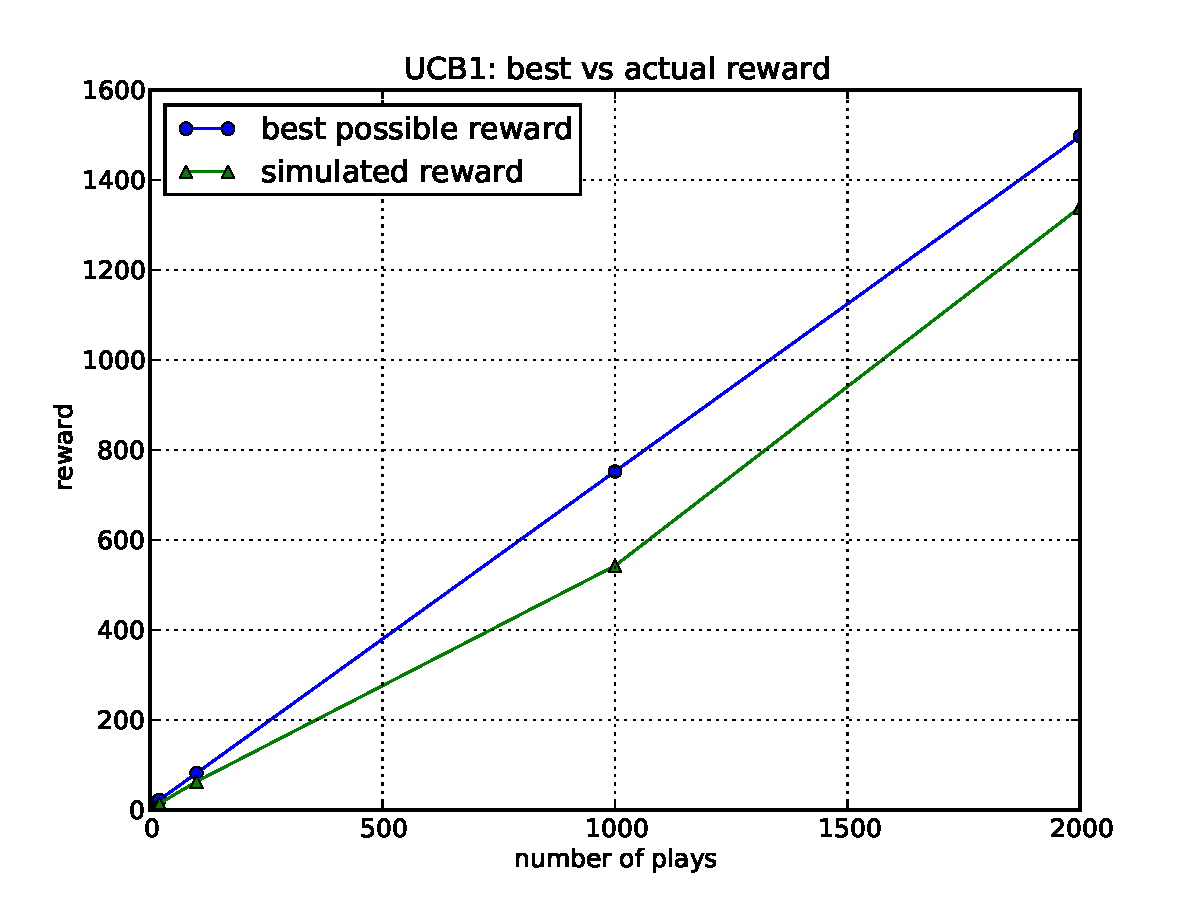
\includegraphics[width=.75\textwidth]{best_and_total_reward.pdf}
\end{center}
\caption{Comparing best and actual reward using the UCB1 strategy with
$10$ machines. See Section~\ref{pythonucb} for details on the machines' reward
distributions.}\label{figucbreward}
\end{figure}
%%%%%%%%%%%%%%%%%%%%%%%%%%%
The {\em regret} is the lost reward due to not having played the optimal
machine at each step:
\[
n \mu^* - \mu_j \sum_{j=1}^K \mathbb{E}(T_j(n))
\]
where $T_j(n)$ is the number of times that machine $j$ has been played
after $n$ plays. Importantly, the regret can be bounded to be
logarithmic in the number of plays so far:

\begin{theorem}[\cite{Auer:2002}]\label{thmUCB}
For all $K > 1$, if policy \textnormal{UCB1} is run on $K$ machines
having arbitrary reward distributions $P_1$, \dots, $P_K$ with support
in $[0,1]$ then its expected regret after $n$ plays is at most
\[
\left[ 8 \sum_{i:\mu_i < \mu^*} \left( \frac{\ln n}{\Delta_i} \right)  \right] + 
\left( 1 + \frac{\pi^2}{3} \right)
\left( \sum_{j=1}^K \Delta_j \right)
\]
where $\Delta_i = \mu^* - \mu_i$.
\end{theorem}

Figure~\ref{ucbregret} shows the result of some simulations with $K =
10$ machines and fixed reward distributions.
%%%%%%%%%%%%%%%%%%%%%%%%%%%%%%%%%%%%%
\begin{figure}[htb]
\begin{center}
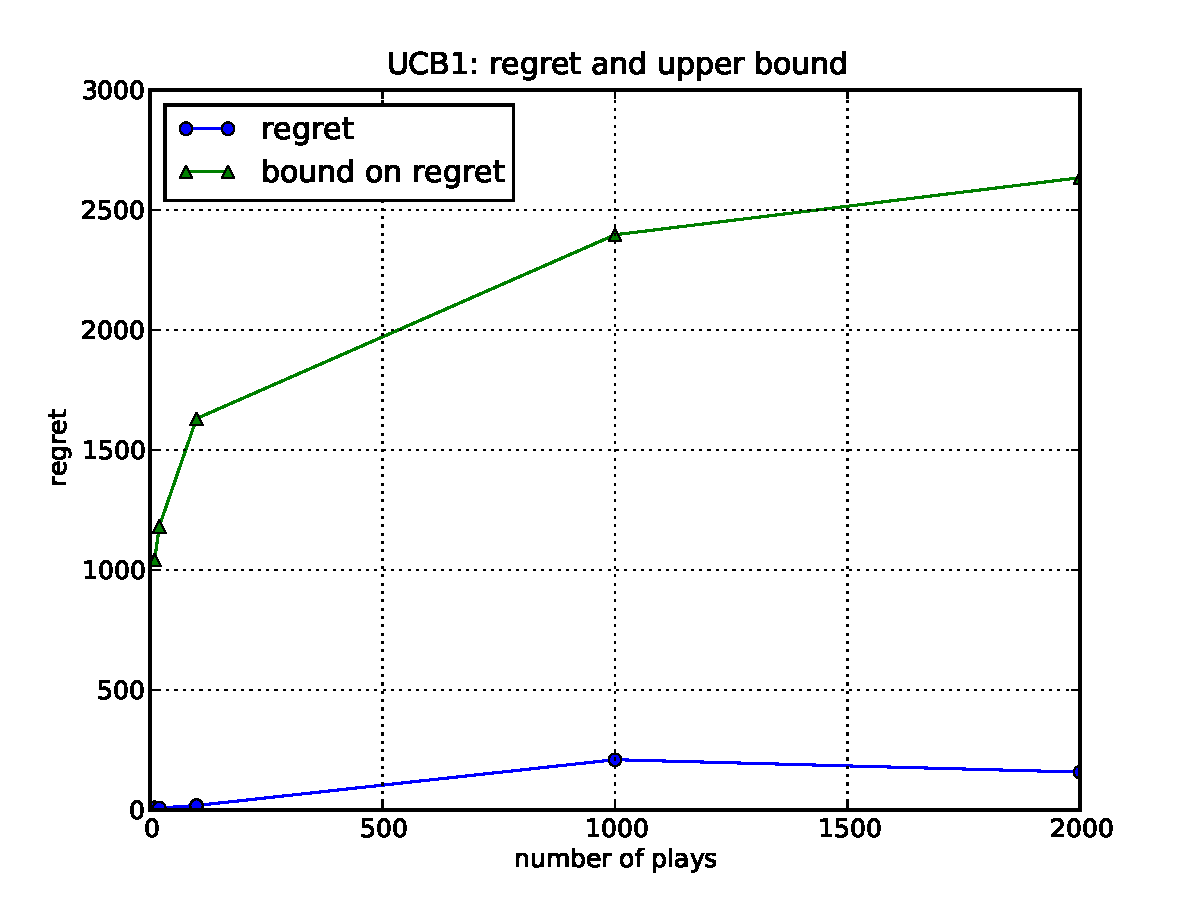
\includegraphics[width=.75\textwidth]{regret_and_bound.pdf}
\end{center}
\caption{Regret and upper bound on regret given by Theorem~\ref{thmUCB}}\label{ucbregret}
\end{figure}
%%%%%%%%%%%%%%%%%%%%%%%%%%%%%%%%%%%%%

\subsection{UCT}

The UCT algorithm is the same as Monte Carlo planning except that UCB is used to
select the action at each tree node. To do this we have to keep track of
the average cost so far (i.e. up to time $t$)
of taking action $a$ from state $s$,
denoted $Q_t(s,a)$. We also track $N_{s}(t)$, the number of times
that state $s$ has been visited up to time $t$. If we are
at a tree node $s$ then the action is chosen using
the UCB rule
\begin{equation}\label{eqnuct}
a^* = \underset{a \in A}{\operatorname{argmax}} 
 \left\{ Q_t(s,a) + \alpha \sqrt{\frac{\ln N_{s}(t)}{N_{s,a}(t)}} \, \right\}.
\end{equation}
where $\alpha$ is a constant that has to be chosen empirically. A badly
chosen $\alpha$ can have a huge effect on the convergence of the
algorithm.

See Section~\ref{pythonuct} for Python source code that uses UCT to
solve the sailing problem.\footnote{I asked the authors of
\cite{Kocsis06banditbased} for their full list of parameter values and source code
but got no reply. If anyone improves my code I will be happy to update
this document and give a reference or URL.}

\subsection{UCT on the sailing problem}

First we used value iteration to solve the sailing problem on lakes of size
$5 \times 5$,
$10 \times 10$, $20 \times 20$,
and $30 \times 30$, with $\varepsilon =
0.01$ (solving just the $20 \times 20$ instance took about 5
hours on a 2.5Ghz Intel Xeon server).
The optimal value and policy vectors $V^*$ and $\pi^*$ 
are available in the pickled Python format as
{\texttt lake\_5.pkl},
{\texttt lake\_10.pkl},
{\texttt lake\_20.pkl}, and
{\texttt lake\_30.pkl}.

Next, we chose $20$ random points (excluding the target point). For
each of these states $s$, we ran the Monte Carlo and UCT algorithm until the estimated
cost for sailing from $s$ to the target state was within $0.1$ of the
optimal value $V^*(s)$. A good measure of the efficiency of a Monte Carlo type of planning
algorithm is the total number of samples taken from the underlying MDP's
generative model. Figure~\ref{uctsailing} shows the number of samples
required to get the estimated error to within the bounds specified.
%%%%%%%%%%%%%%%%%%%%%%%%%%%
\begin{figure}[htb]
\begin{center}
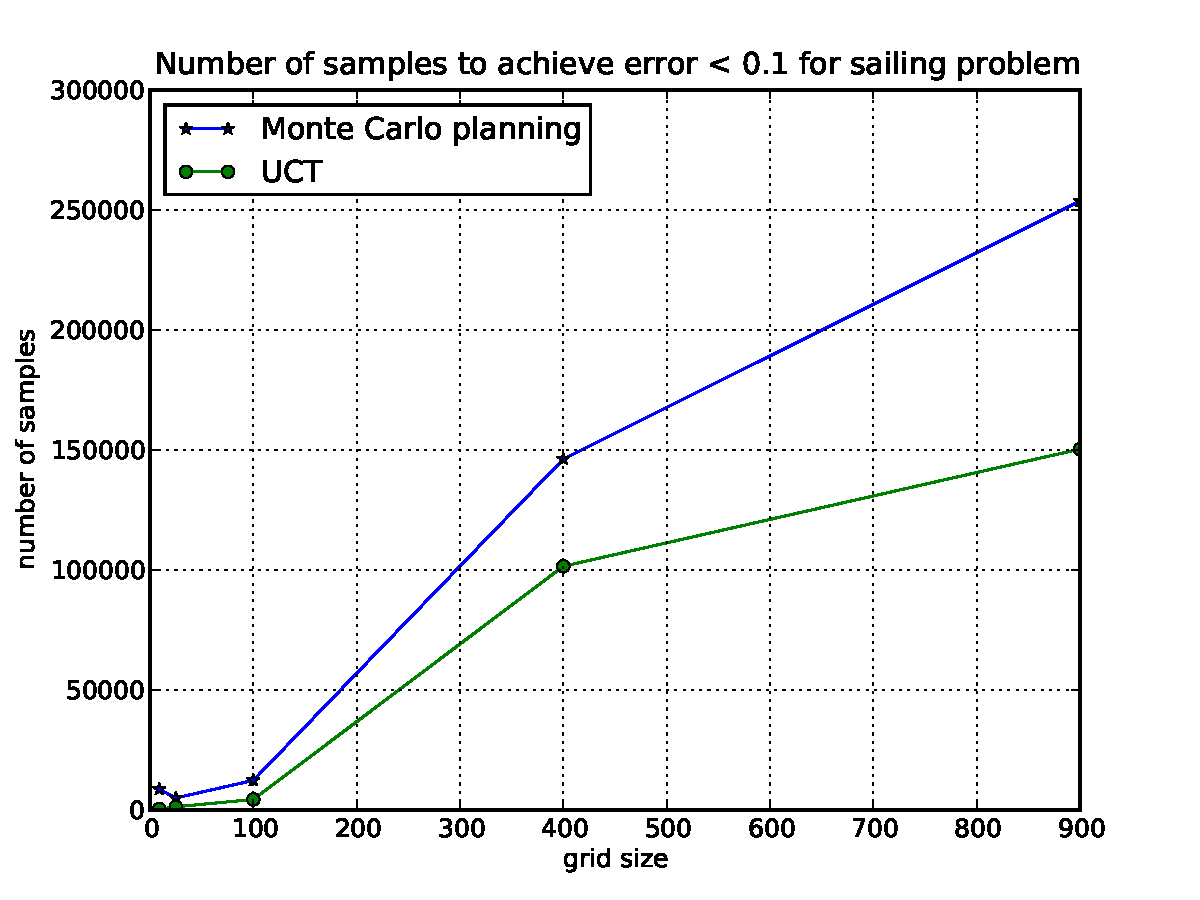
\includegraphics[width=.75\textwidth]{nr_samples_uct_sailing.pdf}
\end{center}
\caption{Performance of plain Monte Carlo planning and UCT on the
sailing problem.}\label{uctsailing}
\end{figure}
%%%%%%%%%%%%%%%%%%%%%%%%%%%

\section{What else?}

There are a few factors that have to be chosen by hand in {\texttt
sailing\_uct.py}. If we are working on a huge problem, where value
iteration isn't feasible, how do we know if we are converging to the
optimal solution? The $0.1$ factor for the $Q$ value update step in
Section~\ref{uctsec} is meant to decay to zero if we want convergence.
But at what rate? Using something like $1/n$ works badly
on the sailing domain with lake sizes up to $20 \times 20$.

Also, there are many ways to improve the UCT algorithm, for example
combining online and offline data to speed up convergence of the $Q$
values: \cite{citeulike:2976742}.

\clearpage
\section{iPod value iteration}\label{secipodpython}

Here is \texttt{ipod\_mdp.py}, also available at\\
\url{http://carlo-hamalainen.net/stuff/mdpnotes}

\begin{Verbatim}[commandchars=@\[\]]
@PYaE[# -*- coding: utf-8 -*-]

@PYaE[#*****************************************************************************]
@PYaE[#       Copyright (C) 2009 Carlo Hamalainen <carlo.hamalainen@at[]gmail.com>, ]
@PYaE[#]
@PYaE[#  Distributed under the terms of the GNU General Public License (GPL)]
@PYaE[#]
@PYaE[#    This code is distributed in the hope that it will be useful,]
@PYaE[#    but WITHOUT ANY WARRANTY; without even the implied warranty of]
@PYaE[#    MERCHANTABILITY or FITNESS FOR A PARTICULAR PURPOSE.  See the GNU]
@PYaE[#    General Public License for more details.]
@PYaE[#]
@PYaE[#  The full text of the GPL is available at:]
@PYaE[#]
@PYaE[#                  http://www.gnu.org/licenses/]
@PYaE[#*****************************************************************************]

@PYas["""]
@PYas[A Markov Decision Process (MDP) for the iPod problem ]
@PYas[described at http://norvig.com/ipod.html]
@PYas["""]

@PYay[import] @PYaV[random]
@PYay[import] @PYaV[sys]

@PYay[def] @PYaL[value_iteration](N, T, target, epsilon @PYbd[=] @PYaw[0.001]):
    @PYaE[# The possible actions from any state:]
    actions @PYbd[=] @lb[]@PYaB[']@PYaB[sequential]@PYaB['], @PYaB[']@PYaB[shuffle]@PYaB[']@rb[]

    @PYaE[# Transition probabilities:]
    @PYaE[# transitions@lb[]s, a, w@rb[] = probability of moving from s to w by action a.]

    transitions @PYbd[=] {}

    @PYaE[# Sequential strategy gets us to the target directly.]
    @PYay[for] s @PYav[in] @PYaX[range](N):
        @PYay[for] w @PYav[in] @PYaX[range](N):
            @PYay[if] w @PYbd[==] target:
                transitions@lb[]s, @PYaB[']@PYaB[sequential]@PYaB['], w@rb[] @PYbd[=] @PYaw[1.0]
            @PYay[else]:
                transitions@lb[]s, @PYaB[']@PYaB[sequential]@PYaB['], w@rb[] @PYbd[=] @PYaw[0.0]

    @PYaE[# The Shuffle strategy takes us to any state with equal]
    @PYaE[# probability.]
    @PYay[for] s @PYav[in] @PYaX[range](N):
        @PYay[for] w @PYav[in] @PYaX[range](N):
            transitions@lb[]s, @PYaB[']@PYaB[shuffle]@PYaB['], w@rb[] @PYbd[=] @PYaw[1.0]@PYbd[/]N

    @PYaE[# Cost of each action from any state s.]
    cost @PYbd[=] {}
    @PYay[for] s @PYav[in] @PYaX[range](N): cost@lb[]s, @PYaB[']@PYaB[sequential]@PYaB[']@rb[] @PYbd[=] @PYaX[abs](target @PYbd[-] s)
    @PYay[for] s @PYav[in] @PYaX[range](N): cost@lb[]s, @PYaB[']@PYaB[shuffle]@PYaB[']@rb[] @PYbd[=] T

    V1 @PYbd[=] @lb[]@PYaw[0]@rb[] @PYbd[*] N
    V2 @PYbd[=] @lb[]@PYaw[1]@rb[] @PYbd[*] N
    policy @PYbd[=] @lb[]@PYaB[']@PYaB[shuffle]@PYaB[']@rb[] @PYbd[*] N

    @PYay[while] @PYaX[max](@lb[]@PYaX[abs](V1@lb[]i@rb[] @PYbd[-] V2@lb[]i@rb[]) @PYay[for] i @PYav[in] @PYaX[range](N)@rb[]) @PYbd[>] epsilon:
        @PYay[for] s @PYav[in] @PYaX[range](N):
            min_action @PYbd[=] actions@lb[]@PYaw[0]@rb[]
            min_action_cost @PYbd[=] cost@lb[]s, actions@lb[]@PYaw[0]@rb[]@rb[] \
                @PYbd[+] @PYaX[sum](@lb[]transitions@lb[]s, actions@lb[]@PYaw[0]@rb[], w@rb[]@PYbd[*]V1@lb[]w@rb[] @PYay[for] w @PYav[in] @PYaX[range](N)@rb[])

            @PYay[for] a @PYav[in] actions:
                this_cost @PYbd[=] cost@lb[]s, a@rb[] @PYbd[+] @PYaX[sum](@lb[]transitions@lb[]s, a, w@rb[]@PYbd[*]V1@lb[]w@rb[] \
                    @PYay[for] w @PYav[in] @PYaX[range](N)@rb[])

                @PYay[if] this_cost @PYbd[<] min_action_cost:
                    min_action @PYbd[=] a
                    min_action_cost @PYbd[=] this_cost

            V2@lb[]s@rb[] @PYbd[=] min_action_cost
            policy@lb[]s@rb[] @PYbd[=] min_action

        V1, V2 @PYbd[=] V2, V1   @PYaE[# swapsies]

    @PYay[try]:
        p @PYbd[=] @PYaX[min](@lb[]s @PYay[for] s @PYav[in] @PYaX[range](N) @PYay[if] policy@lb[]s@rb[] @PYbd[==] @PYaB[']@PYaB[sequential]@PYaB[']@rb[]) @PYbd[-] @PYaw[1]
        q @PYbd[=] @PYaX[min](@lb[]s @PYay[for] s @PYav[in] @PYaX[range](N) @PYay[if] V2@lb[]s@rb[] @PYbd[==] target @PYbd[-] s@rb[]) @PYbd[-] @PYaw[1]

        @PYaE[# fixme: fails if epsilon is too large, ie. our policy vector isn't]
        @PYaE[# optimal.]
        @PYaE[# assert p == q]

        p @PYbd[=] @PYaX[min](@lb[]s @PYay[for] s @PYav[in] @PYaX[range](N) @PYay[if] V2@lb[]s@rb[] @PYbd[==] target @PYbd[-] s@rb[]) @PYbd[-] @PYaw[1]

        @PYay[assert] policy@lb[]p@rb[] @PYbd[==] @PYaB[']@PYaB[shuffle]@PYaB[']
        @PYay[assert] V2@lb[]p@rb[] @PYbd[!=] target @PYbd[-] p

        @PYay[assert] policy@lb[]p @PYbd[+] @PYaw[1]@rb[] @PYbd[==] @PYaB[']@PYaB[sequential]@PYaB[']
        @PYay[assert] V2@lb[]p @PYbd[+] @PYaw[1]@rb[] @PYbd[==] target @PYbd[-] (p @PYbd[+] @PYaw[1])

        @PYay[assert] policy@lb[]p @PYbd[+] @PYaw[2]@rb[] @PYbd[==] @PYaB[']@PYaB[sequential]@PYaB[']
        @PYay[assert] V2@lb[]p @PYbd[+] @PYaw[2]@rb[] @PYbd[==] target @PYbd[-] (p @PYbd[+] @PYaw[2])
    @PYay[except] @PYbe[ValueError]:
        @PYaE[# we must have come in with a high epsilon value and didn't get]
        @PYaE[# a 'correct' value/policy vector.]
        p @PYbd[=] @PYaA[None]

    @PYay[return] V2, policy, p

@PYay[def] @PYaL[simulate](N, T, initial_state, target, policy):
    s @PYbd[=] initial_state
    total_cost @PYbd[=] @PYaw[0]

    @PYay[while] s @PYbd[!=] target:
        @PYay[if] policy@lb[]s@rb[] @PYbd[==] @PYaB[']@PYaB[sequential]@PYaB[']:
            total_cost @PYbd[+]@PYbd[=] @PYaX[abs](target @PYbd[-] s)
            s @PYbd[=] target
        @PYay[else]: @PYaE[# policy@lb[]s@rb[] == 'shuffle']
            total_cost @PYbd[+]@PYbd[=] T
            s @PYbd[=] random@PYbd[.]randrange(N)

    @PYay[return] total_cost

@PYay[def] @PYaL[average_simulation](N, T, policy):
    @PYaE[# The target state:]
    target @PYbd[=] N@PYbd[/]@PYaw[2]

    nr_iters @PYbd[=] @PYaw[1000]@PYbd[*]N

    @PYay[return] @PYaX[sum](@lb[]simulate(N, T, random@PYbd[.]randrange(N), target, policy) \
        @PYay[for] _ @PYav[in] @PYaX[range](nr_iters)@rb[])@PYbd[/]@PYaX[float](nr_iters)

@PYay[def] @PYaL[usage]():
    @PYay[print]
    @PYay[print] @PYaB["]@PYaB[Usage:]@PYaB["]
    @PYay[print] @PYaB["]@PYaB[$ python ipod_mdp.py <N> <T>]@PYaB["]
    @PYay[print]
    sys@PYbd[.]exit(@PYaw[0])


@PYay[if] __name__ @PYbd[==] @PYaB["]@PYaB[__main__]@PYaB["]:
    @PYay[if] @PYaX[len](sys@PYbd[.]argv) @PYbd[==] @PYaw[1]: usage()

    @PYay[if] @PYaX[len](sys@PYbd[.]argv) @PYbd[==] @PYaw[3]:
        N @PYbd[=] @PYaX[int](sys@PYbd[.]argv@lb[]@PYaw[1]@rb[]) 
        T @PYbd[=] @PYaX[float](sys@PYbd[.]argv@lb[]@PYaw[2]@rb[]) 

        V, policy, p @PYbd[=] value_iteration(N, T, N@PYbd[/]@PYaw[2])

        away @PYbd[=] N@PYbd[/]@PYaw[2] @PYbd[-] p

        @PYay[assert] policy@lb[]N@PYbd[/]@PYaw[2] @PYbd[-] (away @PYbd[-] @PYaw[1])@rb[] @PYbd[==] @PYaB[']@PYaB[sequential]@PYaB[']
        @PYay[assert] policy@lb[]N@PYbd[/]@PYaw[2] @PYbd[-] (away)@rb[] @PYbd[==] @PYaB[']@PYaB[shuffle]@PYaB[']
        @PYay[assert] policy@lb[]N@PYbd[/]@PYaw[2] @PYbd[-] (away @PYbd[+] @PYaw[1])@rb[] @PYbd[==] @PYaB[']@PYaB[shuffle]@PYaB[']

        mean_V @PYbd[=] @PYaX[float](@PYaX[sum](V))@PYbd[/]@PYaX[float](@PYaX[len](V))
        mean_sim @PYbd[=] average_simulation(N, T, policy)

        @PYay[print] @PYaB["]@PYaB[mean(V) =]@PYaB["], mean_V
        @PYay[print] @PYaB["]@PYaB[mean (simulation):]@PYaB["], mean_sim
        @PYay[print] @PYaB["]@PYaB[difference:]@PYaB["], mean_V @PYbd[-] mean_sim

        @PYay[print] @PYaB["]@PYaB[shuffle when:]@PYaB["], away, @PYaB["]@PYaB[or more away]@PYaB["]

        sys@PYbd[.]exit(@PYaw[0])

    usage()
\end{Verbatim}


\clearpage
\section{Value iteration for sailing}\label{pythonsailing}

Here is \texttt{sailing.py}, also available at\\
\url{http://carlo-hamalainen.net/stuff/mdpnotes}

\begin{Verbatim}[commandchars=@\[\]]
@PYaE[# -*- coding: utf-8 -*-]

@PYaE[#*****************************************************************************]
@PYaE[#       Copyright (C) 2009 Carlo Hamalainen <carlo.hamalainen@at[]gmail.com>, ]
@PYaE[#]
@PYaE[#  Distributed under the terms of the GNU General Public License (GPL)]
@PYaE[#]
@PYaE[#    This code is distributed in the hope that it will be useful,]
@PYaE[#    but WITHOUT ANY WARRANTY; without even the implied warranty of]
@PYaE[#    MERCHANTABILITY or FITNESS FOR A PARTICULAR PURPOSE.  See the GNU]
@PYaE[#    General Public License for more details.]
@PYaE[#]
@PYaE[#  The full text of the GPL is available at:]
@PYaE[#]
@PYaE[#                  http://www.gnu.org/licenses/]
@PYaE[#*****************************************************************************]


@PYaE[# For debugging, put these lines somewhere to drop into an ipython shell:]
@PYaE[#import IPython]
@PYaE[#IPython.Shell.IPShell(user_ns=dict(globals(), **locals())).mainloop()]

@PYaE[# To profile, put these in __main__():]
@PYaE[#import cProfile]
@PYaE[#cProfile.run('thing_to_run()')]

@PYay[import] @PYaV[math]
@PYay[import] @PYaV[pickle]
@PYay[import] @PYaV[random]
@PYay[import] @PYaV[sys]

@PYay[from] @PYaV[scipy] @PYay[import] @PYaj[arange], @PYaj[log], logn
@PYay[from] @PYaV[scipy.stats] @PYay[import] rv_discrete

@PYay[def] @PYaL[mean](L): @PYay[return] @PYaX[sum](L)@PYbd[/](@PYaw[1.0]@PYbd[*]@PYaX[len](L))

@PYay[def] @PYaL[stddev](values, meanval@PYbd[=]@PYaA[None]):
    @PYaE[# copied from http://aima.cs.berkeley.edu/python/utils.html]
    @PYaE[# and fixed the denominator.]
    @PYas["""The standard deviation of a set of values.]
@PYas[    Pass in the mean if you already know it."""]
    @PYay[if] meanval @PYbd[==] @PYaA[None]: meanval @PYbd[=] @PYaj[mean](values)
    @PYay[return] math@PYbd[.]@PYaj[sqrt](@PYaX[sum](@lb[](x @PYbd[-] meanval)@PYbd[*]@PYbd[*]@PYaw[2] @PYay[for] x @PYav[in] values@rb[]) @PYbd[/] (@PYaX[len](values)))

@PYay[def] @PYaL[median](values):
    @PYaE[# copied from http://aima.cs.berkeley.edu/python/utils.html]
    @PYas["""Return the middle value, when the values are sorted.]
@PYas[    If there are an odd number of elements, try to average the middle two.]
@PYas[    If they can't be averaged (e.g. they are strings), choose one at random.]
@PYas[    >>> median(@lb[]10, 100, 11@rb[])]
@PYas[    11]
@PYas[    >>> median(@lb[]1, 2, 3, 4@rb[])]
@PYas[    2.5]
@PYas[    """]
    n @PYbd[=] @PYaX[len](values)
    values @PYbd[=] sorted(values)
    @PYay[if] n @PYbd[%] @PYaw[2] @PYbd[==] @PYaw[1]:
        @PYay[return] values@lb[]n@PYbd[/]@PYaw[2]@rb[]
    @PYay[else]:
        middle2 @PYbd[=] values@lb[](n@PYbd[/]@PYaw[2])@PYbd[-]@PYaw[1]:(n@PYbd[/]@PYaw[2])@PYbd[+]@PYaw[1]@rb[]
        @PYay[try]:
            @PYay[return] @PYaj[mean](middle2)
        @PYay[except] @PYbe[TypeError]:
            @PYay[return] random@PYbd[.]choice(middle2)

@PYay[def] @PYaL[my_randint](n):
    @PYas["""]
@PYas[    Return a random integer from @lb[]0, n).]
@PYas[    """]

    @PYay[return] random@PYbd[.]@PYaj[randint](@PYaw[0], n @PYbd[-] @PYaw[1])

@PYay[def] @PYaL[add_vector](x, y, v):
    @PYas["""]
@PYas[    Returns (x + v@lb[]0@rb[], y + v@lb[]1@rb[]).]

@PYas[    EXAMPLES::]

@PYas[        >>> add_vector(0, 0, (0, 1))]
@PYas[        (0, 1)]
@PYas[        >>> add_vector(0, 0, (-2, 1))]
@PYas[        (-2, 1)]
@PYas[    """]
    @PYay[return] (x @PYbd[+] v@lb[]@PYaw[0]@rb[], y @PYbd[+] v@lb[]@PYaw[1]@rb[])

@PYay[def] @PYaL[check_probability_matrix](P):
    @PYas["""]
@PYas[    Rows must sum to 1 and no entry can be negative.]

@PYas[    EXAMPLE::]

@PYas[        >>> wind_array = @lb[] @lb[]0.4, 0.3, 0.0, 0.0, 0.0, 0.0, 0.0, 0.3@rb[], \]
@PYas[                           @lb[]0.4, 0.3, 0.3, 0.0, 0.0, 0.0, 0.0, 0.0@rb[], \]
@PYas[                           @lb[]0.0, 0.4, 0.3, 0.3, 0.0, 0.0, 0.0, 0.0@rb[], \]
@PYas[                           @lb[]0.0, 0.0, 0.4, 0.3, 0.3, 0.0, 0.0, 0.0@rb[], \]
@PYas[                           @lb[]0.0, 0.0, 0.0, 0.4, 0.2, 0.4, 0.0, 0.0@rb[], \]
@PYas[                           @lb[]0.0, 0.0, 0.0, 0.0, 0.3, 0.3, 0.4, 0.0@rb[], \]
@PYas[                           @lb[]0.0, 0.0, 0.0, 0.0, 0.0, 0.3, 0.3, 0.4@rb[], \]
@PYas[                           @lb[]0.4, 0.0, 0.0, 0.0, 0.0, 0.0, 0.3, 0.3@rb[] @rb[]]
@PYas[        >>> check_probability_matrix(wind_array)]
@PYas[        True]
@PYas[    """]

    @PYay[for] x @PYav[in] P:
        @PYay[if] @PYaX[sum](x) @PYbd[!=] @PYaw[1]: @PYay[return] @PYaA[False]

        @PYay[for] y @PYav[in] x:
            @PYay[if] y @PYbd[<] @PYaw[0]: @PYay[return] @PYaA[False]

    @PYay[return] @PYaA[True]

@PYay[def] @PYaL[abs_direction_difference](d1, d2):
    @PYas["""]
@PYas[    Absolute difference in directions.]

@PYas[    EXAMPLES::]

@PYas[        >>> abs_direction_difference(0, 1)]
@PYas[        1]
@PYas[        >>> abs_direction_difference(3, 2)]
@PYas[        1]
@PYas[        >>> abs_direction_difference(3, 5)]
@PYas[        2]
@PYas[        >>> abs_direction_difference(3, 7)]
@PYas[        4]
@PYas[    """]

    @PYay[assert] d1 @PYbd[>]@PYbd[=] @PYaw[0]
    @PYay[assert] d1 @PYbd[<] @PYaw[8]

    @PYay[assert] d2 @PYbd[>]@PYbd[=] @PYaw[0]
    @PYay[assert] d2 @PYbd[<] @PYaw[8]

    x @PYbd[=] @PYaX[abs](d1 @PYbd[-] d2)

    @PYay[if] x @PYbd[<] @PYaw[8] @PYbd[-] x:   @PYay[return] x
    @PYay[else]:           @PYay[return] @PYaw[8] @PYbd[-] x

@PYay[def] @PYaL[tack](boat_direction, wind_direction):
    @PYas["""]
@PYas[    The tack of the boat depends on the relative difference of]
@PYas[    the boat's direction and the wind.]

@PYas[    EXAMPLES::]

@PYas[        >>> tack(0, 0)]
@PYas[        'away']
@PYas[        >>> tack(0, 7)]
@PYas[        'down']
@PYas[        >>> tack(0, 2)]
@PYas[        'cross']
@PYas[        >>> tack(0, 3)]
@PYas[        'up']
@PYas[        >>> tack(0, 4)]
@PYas[        'into']
@PYas[    """]

    @PYay[assert] boat_direction @PYbd[>]@PYbd[=] @PYaw[0]
    @PYay[assert] boat_direction @PYbd[<] @PYaw[8]

    @PYay[assert] wind_direction @PYbd[>]@PYbd[=] @PYaw[0]
    @PYay[assert] wind_direction @PYbd[<] @PYaw[8]

    d @PYbd[=] abs_direction_difference(boat_direction, wind_direction)

    @PYay[if] d @PYbd[==] @PYaw[0]: @PYay[return] @PYaB[']@PYaB[away]@PYaB[']
    @PYay[if] d @PYbd[==] @PYaw[1]: @PYay[return] @PYaB[']@PYaB[down]@PYaB[']
    @PYay[if] d @PYbd[==] @PYaw[2]: @PYay[return] @PYaB[']@PYaB[cross]@PYaB[']
    @PYay[if] d @PYbd[==] @PYaw[3]: @PYay[return] @PYaB[']@PYaB[up]@PYaB[']
    @PYay[if] d @PYbd[==] @PYaw[4]: @PYay[return] @PYaB[']@PYaB[into]@PYaB[']

    @PYay[raise] @PYbe[ValueError]

@PYay[def] @PYaL[wind_on_left](boat_dirn, wind_dirn):
    @PYas["""]
@PYas[    Relative to the boat, is the wind blowing to the left of the boat?]
@PYas[    """]

    @PYaE[# If the boat had been going north then we just need to check ]
    @PYaE[# if the wind direction is in @lb[]5, 6, 7@rb[]]

    w @PYbd[=] wind_dirn @PYbd[-] boat_dirn

    @PYay[while] w @PYbd[<] @PYaw[0]: w @PYbd[+]@PYbd[=] @PYaw[8]

    @PYay[return] w @PYav[in] @lb[]@PYaw[5], @PYaw[6], @PYaw[7]@rb[]

@PYay[def] @PYaL[direction_vector](d):
    @PYas["""]
@PYas[    The direction 0 is north so we move by (0, 1) in cartesian]
@PYas[    coordinates.]

@PYas[    EXAMPLES::]

@PYas[        >>> direction_vector(0) # north]
@PYas[        (0, 1)]
@PYas[        >>> direction_vector(6) # west]
@PYas[        (-1, 0)]
@PYas[    """]

    @PYay[assert] d @PYbd[>]@PYbd[=] @PYaw[0]
    @PYay[assert] d @PYbd[<] @PYaw[8]

    @PYay[if] d @PYbd[==] @PYaw[0]: @PYay[return] (@PYaw[0], @PYaw[1])
    @PYay[if] d @PYbd[==] @PYaw[1]: @PYay[return] (@PYaw[1], @PYaw[1])
    @PYay[if] d @PYbd[==] @PYaw[2]: @PYay[return] (@PYaw[1], @PYaw[0])
    @PYay[if] d @PYbd[==] @PYaw[3]: @PYay[return] (@PYaw[1], @PYbd[-]@PYaw[1])
    @PYay[if] d @PYbd[==] @PYaw[4]: @PYay[return] (@PYaw[0], @PYbd[-]@PYaw[1])
    @PYay[if] d @PYbd[==] @PYaw[5]: @PYay[return] (@PYbd[-]@PYaw[1], @PYbd[-]@PYaw[1])
    @PYay[if] d @PYbd[==] @PYaw[6]: @PYay[return] (@PYbd[-]@PYaw[1], @PYaw[0])
    @PYay[if] d @PYbd[==] @PYaw[7]: @PYay[return] (@PYbd[-]@PYaw[1], @PYaw[1])

@PYay[class] @PYaO[Sailing]:
    @PYay[def] @PYaL[__init__](@PYaA[self], lake_size):
        @PYaA[self]@PYbd[.]gamma @PYbd[=] @PYaw[0.9] @PYaE[# discounting factor]

        @PYaA[self]@PYbd[.]lake_size @PYbd[=] lake_size

        @PYaE[# Wind transition probabilities.]
        @PYaA[self]@PYbd[.]wind_array @PYbd[=] @lb[] \
            @lb[]@PYaw[0.4], @PYaw[0.3], @PYaw[0.0], @PYaw[0.0], @PYaw[0.0], @PYaw[0.0], @PYaw[0.0], @PYaw[0.3]@rb[], \
            @lb[]@PYaw[0.4], @PYaw[0.3], @PYaw[0.3], @PYaw[0.0], @PYaw[0.0], @PYaw[0.0], @PYaw[0.0], @PYaw[0.0]@rb[], \
            @lb[]@PYaw[0.0], @PYaw[0.4], @PYaw[0.3], @PYaw[0.3], @PYaw[0.0], @PYaw[0.0], @PYaw[0.0], @PYaw[0.0]@rb[], \
            @lb[]@PYaw[0.0], @PYaw[0.0], @PYaw[0.4], @PYaw[0.3], @PYaw[0.3], @PYaw[0.0], @PYaw[0.0], @PYaw[0.0]@rb[], \
            @lb[]@PYaw[0.0], @PYaw[0.0], @PYaw[0.0], @PYaw[0.4], @PYaw[0.2], @PYaw[0.4], @PYaw[0.0], @PYaw[0.0]@rb[], \
            @lb[]@PYaw[0.0], @PYaw[0.0], @PYaw[0.0], @PYaw[0.0], @PYaw[0.3], @PYaw[0.3], @PYaw[0.4], @PYaw[0.0]@rb[], \
            @lb[]@PYaw[0.0], @PYaw[0.0], @PYaw[0.0], @PYaw[0.0], @PYaw[0.0], @PYaw[0.3], @PYaw[0.3], @PYaw[0.4]@rb[], \
            @lb[]@PYaw[0.4], @PYaw[0.0], @PYaw[0.0], @PYaw[0.0], @PYaw[0.0], @PYaw[0.0], @PYaw[0.3], @PYaw[0.3]@rb[] \
        @rb[]

        @PYaA[self]@PYbd[.]end_x @PYbd[=] lake_size @PYbd[-] @PYaw[1]
        @PYaA[self]@PYbd[.]end_y @PYbd[=] lake_size @PYbd[-] @PYaw[1]

        @PYaA[self]@PYbd[.]costs @PYbd[=] { @PYaB[']@PYaB[up]@PYaB[']:@PYaw[4], @PYaB[']@PYaB[cross]@PYaB[']:@PYaw[3], @PYaB[']@PYaB[down]@PYaB[']:@PYaw[2], @PYaB[']@PYaB[away]@PYaB[']:@PYaw[1] }

        @PYaA[self]@PYbd[.]wind_distribution @PYbd[=] @lb[]@rb[]
        @PYay[for] i @PYav[in] @PYaX[range](@PYaX[len](@PYaA[self]@PYbd[.]wind_array)):
            vals @PYbd[=] @lb[]@PYaj[arange](@PYaX[len](@PYaA[self]@PYbd[.]wind_array@lb[]i@rb[])), @PYaA[self]@PYbd[.]wind_array@lb[]i@rb[]@rb[]
            @PYaA[self]@PYbd[.]wind_distribution@PYbd[.]@PYaj[append](rv_discrete(name@PYbd[=]@PYaB[']@PYaB[custm]@PYaB['], \
                                                    values@PYbd[=]vals))

    @PYay[def] @PYaL[states](@PYaA[self]):
        @PYas["""]
@PYas[        Instead of storing the states in a large list/dictionary, we]
@PYas[        provide an iterator.]
@PYas[        """]

        @PYay[for] x @PYav[in] @PYaX[range](@PYaA[self]@PYbd[.]lake_size):
            @PYay[for] y @PYav[in] @PYaX[range](@PYaA[self]@PYbd[.]lake_size):
                @PYay[for] d @PYav[in] @PYaX[range](@PYaw[8]):
                    @PYay[for] w1 @PYav[in] @PYaX[range](@PYaw[8]):
                        @PYay[for] w2 @PYav[in] @PYaX[range](@PYaw[8]):
                            @PYay[yield] (x, y, d, w1, w2)

    @PYay[def] @PYaL[is_terminal](@PYaA[self], state):
        @PYay[return] (state@lb[]@PYaw[0]@rb[], state@lb[]@PYaw[1]@rb[]) @PYbd[==] (@PYaA[self]@PYbd[.]end_x, @PYaA[self]@PYbd[.]end_y)

    @PYay[def] @PYaL[is_into](@PYaA[self], state, action):
        @PYay[try]:
            @PYaA[self]@PYbd[.]cost(state, action)
        @PYay[except] @PYbe[KeyError]:
            @PYay[return] @PYaA[True]

        @PYay[return] @PYaA[False]

    @PYay[def] @PYaL[random_state](@PYaA[self]):
        w1 @PYbd[=] my_randint(@PYaw[8])
        @PYay[while] @PYaA[True]: @PYaE[# we weren't sailing into the wind...]
            d @PYbd[=] my_randint(@PYaw[8])
            @PYay[if] tack(d, w1) @PYbd[!=] @PYaB[']@PYaB[into]@PYaB[']: @PYay[break]
        w2 @PYbd[=] @PYaA[self]@PYbd[.]new_wind(w1)

        @PYay[while] @PYaA[True]:
            state @PYbd[=] (my_randint(@PYaA[self]@PYbd[.]lake_size), my_randint(@PYaA[self]@PYbd[.]lake_size), d, w1, w2)
            @PYay[if] @PYav[not] @PYaA[self]@PYbd[.]is_terminal(state): @PYay[break]

        @PYay[return] state


    @PYay[def] @PYaL[stays_in_lake](@PYaA[self], state, action):
        x, y, _, _, _ @PYbd[=] state
        x2, y2 @PYbd[=] add_vector(x, y, direction_vector(action))

        @PYay[if] x2 @PYav[in] @PYaX[range](@PYaA[self]@PYbd[.]lake_size) @PYav[and] y2 @PYav[in] @PYaX[range](@PYaA[self]@PYbd[.]lake_size):
            @PYay[return] @PYaA[True]

        @PYay[return] @PYaA[False]

    @PYay[def] @PYaL[average_cost_of_transition](@PYaA[self], V, s, new_d):
        x, y, _, _, w2 @PYbd[=] s

        x2, y2 @PYbd[=] add_vector(x, y, direction_vector(new_d))

        @PYay[if] @PYav[not] @PYaA[self]@PYbd[.]stays_in_lake(s, new_d): @PYay[return] @PYaA[None]

        this_cost @PYbd[=] @PYaw[0]

        @PYaE[# We perform the local action]
        @PYay[try]:
            this_cost @PYbd[+]@PYbd[=] @PYaA[self]@PYbd[.]cost(s, new_d)
        @PYay[except] @PYbe[KeyError]:
            @PYaE[# don't sail into the wind...]
            @PYay[return] @PYaA[None]

        @PYay[for] w3 @PYav[in] @PYaX[range](@PYaw[8]):
            s_new @PYbd[=] (x2, y2, new_d, w2, w3)

            this_cost @PYbd[+]@PYbd[=] @PYaA[self]@PYbd[.]gamma@PYbd[*]@PYaA[self]@PYbd[.]transition_probability(s, s_new)@PYbd[*]V@lb[]s_new@rb[] 

        @PYay[return] this_cost

    @PYay[def] @PYaL[transition_probability](@PYaA[self], s1, s2):
        @PYas["""]
@PYas[        What is the probability of moving from state s1 to s2?]

@PYas[        s1 = (x1, y1, _, w1, w2)]
@PYas[        s2 = (x2, y2, d2, w2_2, w3)]

@PYas[        The boat was at (x1, y1) and travelled to (x2, y2). Then it must]
@PYas[        be the case that (x2, y2) = (x1, y1) + direction_vector(d2). If this]
@PYas[        does not hold then the probability is 0.]

@PYas[        If the previous wind direction of s2 does not match the new]
@PYas[        wind direction of s1 then the probability is 0 (so we need ]
@PYas[        w2_2 == w2).]

@PYas[        Finally, the probability of moving from s1 to s2 is just the]
@PYas[        probability of the wind changing from w2=w2_2 to w3, which is ]
@PYas[        stored in the global variable wind_array.]

@PYas[        >>> x1, y1 = 1, 1]
@PYas[        >>> x2, y2 = 2, 1]
@PYas[        >>> d1 = 0]
@PYas[        >>> d2 = 2 # the direction that we just travelled]
@PYas[        >>> w1 = 3]
@PYas[        >>> w2 = 2]
@PYas[        >>> w2_2 = w2]

@PYas[        >>> lake_size = 5]

@PYas[        >>> S = Sailing(lake_size)]

@PYas[        >>> S.transition_probability((x1, y1, d1, w1, w2), \]
@PYas[                                    (x2, y2, d2, w2_2, 1))]
@PYas[        0.40000000000000002]
@PYas[        >>> S.transition_probability((x1, y1, d1, w1, w2), \]
@PYas[                                    (x2, y2, d2, w2_2, 0))]
@PYas[        0.0]
@PYas[        """]

        x1, y1, _, w1, w2 @PYbd[=] s1
        x2, y2, d2, w2_2, w3 @PYbd[=] s2

        d_vec1, d_vec2 @PYbd[=] direction_vector(d2)

        @PYaE[# The boat was at (x1,y1) and travelled in]
        @PYaE[# direction d2 to arrive at (x2, y2).]
        @PYay[if] x2 @PYbd[!=] x1 @PYbd[+] d_vec1: @PYay[return] @PYaw[0]
        @PYay[if] y2 @PYbd[!=] y1 @PYbd[+] d_vec2: @PYay[return] @PYaw[0]

        @PYaE[# The new wind direction for s1 must be the]
        @PYaE[# previous wind direction of s2.]
        @PYay[if] w2 @PYbd[!=] w2_2: @PYay[return] @PYaw[0]

        @PYaE[# Now we just have the probability of going from]
        @PYaE[# wind direction w2 to wind direction w3.]

        @PYay[return] @PYaA[self]@PYbd[.]wind_array@lb[]w2@rb[]@lb[]w3@rb[]

    @PYay[def] @PYaL[new_wind](@PYaA[self], w):
        @PYas["""]
@PYas[        The wind is currently blowing in direction w and it changes to a]
@PYas[        new direction according to the matrix wind_array, which is encoded]
@PYas[        by general probability distribution in wind_probability_space.]

@PYas[        EXAMPLES::]

@PYas[            >>> lake_size = 5]
@PYas[            >>> S = Sailing(lake_size)]
@PYas[            >>> S.new_wind(0) in range(8)]
@PYas[            True]
@PYas[            >>> S.new_wind(4) in range(8)]
@PYas[            True]
@PYas[        """]

        @PYaE[#assert w in range(8)]

        @PYaE[#return self.wind_distribution@lb[]w@rb[].get_random_element()]
        @PYay[return] @PYaA[self]@PYbd[.]wind_distribution@lb[]w@rb[]@PYbd[.]rvs()

    @PYay[def] @PYaL[cost](@PYaA[self], s, d):
        @PYas["""]
@PYas[        If we are in state s and we decide to travel in direction d, how]
@PYas[        much will this cost? Note that the wind for this new leg is in the ]
@PYas[        last element of s.]

@PYas[        EXAMPLES::]

@PYas[            >>> x1, y1 = 1, 1]
@PYas[            >>> x2, y2 = 2, 1]
@PYas[            >>> d1 = 0]
@PYas[            >>> d2 = 2]
@PYas[            >>> w1 = 3]
@PYas[            >>> w2 = 2]
@PYas[            >>> s = (x1, y1, d1, w1, w2)]

@PYas[            >>> lake_size = 5]
@PYas[            >>> S = Sailing(lake_size)]
@PYas[            >>> S.cost(s, 0)]
@PYas[            3]
@PYas[            >>> S.cost(s, 1)]
@PYas[            2]
@PYas[        """]
        new_wind @PYbd[=] s@lb[]@PYbd[-]@PYaw[1]@rb[]

        @PYay[return] @PYaA[self]@PYbd[.]costs@lb[]tack(d, new_wind)@rb[]

    @PYay[def] @PYaL[best_action](@PYaA[self], s, V):
        @PYas["""]
@PYas[        If we are in state s, use the value vector V to work out the]
@PYas[        best direction to travel in and its estimated cost.]
@PYas[        """]

        x, y, d, w1, w2 @PYbd[=] s

        @PYaE[# this is the end state]
        @PYay[if] @PYaA[self]@PYbd[.]is_terminal(s): @PYay[return] (@PYbd[-]@PYaw[1], @PYaw[0]) @PYaE[# (no action, terminal cost)]

        @PYaE[# Otherwise we have to loop through all possible actions]
        @PYaE[# and find the one with the minimum cost.]

        min_d @PYbd[=] @PYaA[None]
        min_d_cost @PYbd[=] @PYaA[None]

        @PYay[for] new_d @PYav[in] @PYaX[range](@PYaw[8]):
            new_d_cost @PYbd[=] @PYaA[self]@PYbd[.]average_cost_of_transition(V, s, new_d)
            @PYay[if] new_d_cost @PYbd[==] @PYaA[None]: @PYay[continue]

            @PYay[if] min_d @PYav[is] @PYaA[None]:
                min_d @PYbd[=] new_d
                min_d_cost @PYbd[=] new_d_cost
            @PYay[elif] new_d_cost @PYbd[<] min_d_cost:
                min_d @PYbd[=] new_d
                min_d_cost @PYbd[=] new_d_cost

        @PYay[return] (min_d, min_d_cost)

    @PYay[def] @PYaL[value_iteration](@PYaA[self], epsilon):
        V1 @PYbd[=] {}
        V2 @PYbd[=] {}
        policy @PYbd[=] {}
        @PYay[for] s @PYav[in] @PYaA[self]@PYbd[.]states():
            V1@lb[]s@rb[] @PYbd[=] @PYaw[0]
            V2@lb[]s@rb[] @PYbd[=] @PYaw[10]@PYbd[*]epsilon
            policy@lb[]s@rb[] @PYbd[=] @PYbd[-]@PYaw[1]

            @PYay[if] @PYaA[self]@PYbd[.]is_terminal(s):
                V1@lb[]s@rb[] @PYbd[=] @PYaw[0]
                V2@lb[]s@rb[] @PYbd[=] @PYaw[0]

        @PYay[while] @PYaA[True]:
            max_diff @PYbd[=] @PYaX[max](@lb[]@PYaX[abs](V1@lb[]i@rb[] @PYbd[-] V2@lb[]i@rb[]) @PYay[for] i @PYav[in] @PYaA[self]@PYbd[.]states()@rb[])
            @PYay[print] @PYaB["]@PYaB[Top of value_iteration(), max difference:]@PYaB["], max_diff
            sys@PYbd[.]stdout@PYbd[.]flush()

            @PYay[if] max_diff @PYbd[<] epsilon: @PYay[break]

            @PYay[for] s @PYav[in] @PYaA[self]@PYbd[.]states():
                @PYay[if] @PYaA[self]@PYbd[.]is_terminal(s): @PYay[continue]

                policy@lb[]s@rb[], V2@lb[]s@rb[] @PYbd[=] @PYaA[self]@PYbd[.]best_action(s, V1)

            V1, V2 @PYbd[=] V2, V1

        V @PYbd[=] V2

        V_avg @PYbd[=] @PYaX[sum](V@PYbd[.]values())@PYbd[/]@PYaX[len](V)
        V_stddev @PYbd[=] stddev(V@PYbd[.]values(), meanval @PYbd[=] V_avg)

        @PYay[return] V, policy, V_avg, V_stddev

    @PYay[def] @PYaL[simulate](@PYaA[self], policy):
        w1 @PYbd[=] my_randint(@PYaw[8])

        @PYaE[# boat not facing into the wind]
        @PYay[while] @PYaA[True]:
            d @PYbd[=] my_randint(@PYaw[8])
            @PYay[if] tack(d, w1) @PYbd[!=] @PYaB[']@PYaB[into]@PYaB[']: @PYay[break]

        w2 @PYbd[=] @PYaA[self]@PYbd[.]new_wind(w1)

        current_state @PYbd[=] (my_randint(@PYaA[self]@PYbd[.]lake_size), my_randint(@PYaA[self]@PYbd[.]lake_size), d, w1, w2)

        this_cost @PYbd[=] @PYaw[0]
        factor @PYbd[=] @PYaw[1.0]

        @PYay[while] @PYav[not] @PYaA[self]@PYbd[.]is_terminal(current_state):
            new_d @PYbd[=] policy@lb[]current_state@rb[]

            this_cost @PYbd[+]@PYbd[=] factor@PYbd[*]@PYaA[self]@PYbd[.]cost(current_state, new_d)

            x2, y2 @PYbd[=] add_vector(current_state@lb[]@PYaw[0]@rb[], current_state@lb[]@PYaw[1]@rb[], \
                direction_vector(new_d))
            w3 @PYbd[=] @PYaA[self]@PYbd[.]new_wind(current_state@lb[]@PYbd[-]@PYaw[1]@rb[])
            current_state @PYbd[=] x2, y2, new_d, current_state@lb[]@PYbd[-]@PYaw[1]@rb[], w3

            factor @PYbd[*]@PYbd[=] @PYaA[self]@PYbd[.]gamma

        @PYay[return] this_cost

    @PYay[def] @PYaL[run_simulations](@PYaA[self], policy, nr_sims):
        sims @PYbd[=] @lb[]@rb[]
        @PYay[for] i @PYav[in] @PYaX[range](@PYaw[1], nr_sims @PYbd[+] @PYaw[1]):
            sims@PYbd[.]@PYaj[append](@PYaA[self]@PYbd[.]simulate(policy))

        sims_avg @PYbd[=] @PYaX[sum](sims)@PYbd[/]@PYaX[len](sims)
        sims_stddev @PYbd[=] stddev(sims, meanval @PYbd[=] sims_avg)

        @PYay[return] sims, sims_avg, sims_stddev

    @PYay[def] @PYaL[sample_next_state](@PYaA[self], state, action):
        @PYas["""]
@PYas[        Use the generative model of S to find the next state given that]
@PYas[        we are in state and take action action.]
@PYas[        """]

        @PYay[if] @PYaA[self]@PYbd[.]is_terminal(state): 
            @PYay[return] @PYaA[None]

        cost @PYbd[=] @PYaA[self]@PYbd[.]cost(state, action)
        x2, y2 @PYbd[=] add_vector(state@lb[]@PYaw[0]@rb[], state@lb[]@PYaw[1]@rb[], direction_vector(action))
        w3 @PYbd[=] @PYaA[self]@PYbd[.]new_wind(state@lb[]@PYbd[-]@PYaw[1]@rb[])
        new_state @PYbd[=] x2, y2, action, state@lb[]@PYbd[-]@PYaw[1]@rb[], w3

        @PYay[return] new_state, cost

@PYay[def] @PYaL[value_iteration_example]():
    lake_size @PYbd[=] @PYaw[5]

    S @PYbd[=] Sailing(lake_size @PYbd[=] lake_size) 
    V, policy, V_avg, V_stddev @PYbd[=] S@PYbd[.]value_iteration(epsilon @PYbd[=] @PYaw[0.1])
    @PYay[print] @PYaB["]@PYaB[Done with value iteration]@PYaB["]

    @PYaE[# Run a few thousand simulations:]
    nr_sims @PYbd[=] @PYaw[1000]
    @PYay[print] @PYaB["]@PYaB[Running simulations...]@PYaB["]
    sims, sims_avg, sims_stddev @PYbd[=] S@PYbd[.]run_simulations(policy, nr_sims)

    @PYay[print]
    @PYay[print] @PYaB["]@PYaB[Lake size: ]@PYbf[%d]@PYaB[ x ]@PYbf[%d]@PYaB["] @PYbd[%] (lake_size, lake_size)
    @PYay[print]
    @PYay[print] @PYaB["]@PYaB[Value iteration:]@PYaB["]
    @PYay[print] @PYaB["]@PYaB[    Mean cost: ]@PYbf[%.1f]@PYaB["] @PYbd[%] V_avg
    @PYay[print] @PYaB["]@PYaB[    Median cost: ]@PYbf[%.1f]@PYaB["] @PYbd[%] @PYaj[median](V@PYbd[.]values())
    @PYay[print] @PYaB["]@PYaB[    Standard dev: ]@PYbf[%.1f]@PYaB["] @PYbd[%] V_stddev
    @PYay[print]
    @PYay[print] @PYaB["]@PYaB[Simulations (run ]@PYbf[%d]@PYaB[ times):]@PYaB["] @PYbd[%] nr_sims
    @PYay[print] @PYaB["]@PYaB[    Mean cost: ]@PYbf[%.1f]@PYaB["] @PYbd[%] sims_avg
    @PYay[print] @PYaB["]@PYaB[    Median cost: ]@PYbf[%.1f]@PYaB["] @PYbd[%] @PYaj[median](sims)
    @PYay[print] @PYaB["]@PYaB[    Standard dev: ]@PYbf[%.1f]@PYaB["] @PYbd[%] sims_stddev

    @PYay[print]
    v_11 @PYbd[=] @PYaw[0.0]
    v_11_count @PYbd[=] @PYaw[0]

    @PYay[for] s @PYav[in] V@PYbd[.]keys():
        @PYay[if] (s@lb[]@PYaw[0]@rb[], s@lb[]@PYaw[1]@rb[]) @PYbd[==] (@PYaw[1], @PYaw[1]):
            v_11_count @PYbd[+]@PYbd[=] @PYaw[1]
            v_11 @PYbd[+]@PYbd[=] V@lb[]s@rb[]

    @PYay[print] @PYaB["]@PYaB[Mean cost to sail across lake from (1, 1) to (]@PYbf[%d]@PYaB[, ]@PYbf[%d]@PYaB[): ]@PYbf[%.1f]@PYaB["] \
        @PYbd[%] (S@PYbd[.]end_x, S@PYbd[.]end_y, (v_11@PYbd[/]v_11_count))

@PYay[def] @PYaL[save_optimal_solution](lake_size):
    S @PYbd[=] Sailing(lake_size)
    V, policy, V_avg, V_stddev @PYbd[=] S@PYbd[.]value_iteration(@PYaw[0.01])

    lake_filename @PYbd[=] @PYaB["]@PYaB[lake_]@PYaB["] @PYbd[+] @PYaX[str](lake_size) @PYbd[+] @PYaB["]@PYaB[.pkl]@PYaB["]

    output @PYbd[=] @PYaX[open](lake_filename, @PYaB[']@PYaB[wb]@PYaB['])
    pickle@PYbd[.]@PYaj[dump](V, output)
    pickle@PYbd[.]@PYaj[dump](policy, output)
    pickle@PYbd[.]@PYaj[dump](V_avg, output)
    pickle@PYbd[.]@PYaj[dump](V_stddev, output)
    output@PYbd[.]close()


@PYay[if] __name__ @PYbd[==] @PYaB["]@PYaB[__main__]@PYaB["]:
    @PYay[if] @PYaX[len](sys@PYbd[.]argv) @PYbd[==] @PYaw[2]:
        @PYaX[eval](sys@PYbd[.]argv@lb[]@PYaw[1]@rb[])
    @PYay[else]:
        value_iteration_example()
\end{Verbatim}


\clearpage
\section{UCB}\label{pythonucb}

Here is \texttt{ucb.py}, also available at\\
\url{http://carlo-hamalainen.net/stuff/mdpnotes}

\begin{Verbatim}[commandchars=@\[\]]
@PYaE[# -*- coding: utf-8 -*-]

@PYaE[#*****************************************************************************]
@PYaE[#       Copyright (C) 2009 Carlo Hamalainen <carlo.hamalainen@at[]gmail.com>, ]
@PYaE[#]
@PYaE[#  Distributed under the terms of the GNU General Public License (GPL)]
@PYaE[#]
@PYaE[#    This code is distributed in the hope that it will be useful,]
@PYaE[#    but WITHOUT ANY WARRANTY; without even the implied warranty of]
@PYaE[#    MERCHANTABILITY or FITNESS FOR A PARTICULAR PURPOSE.  See the GNU]
@PYaE[#    General Public License for more details.]
@PYaE[#]
@PYaE[#  The full text of the GPL is available at:]
@PYaE[#]
@PYaE[#                  http://www.gnu.org/licenses/]
@PYaE[#*****************************************************************************]


@PYay[import] @PYaV[pylab]
@PYay[from] @PYaV[scipy] @PYay[import] @PYaj[arange], @PYaj[log], pi, @PYaj[sqrt]
@PYay[from] @PYaV[scipy.stats] @PYay[import] rv_discrete

@PYay[def] @PYaL[avg](L): @PYay[return] @PYaX[sum](L)@PYbd[/](@PYaw[1.0]@PYbd[*]@PYaX[len](L))

@PYay[def] @PYaL[make_scipy_rv](L):
    vals @PYbd[=] @lb[]@PYaj[arange](@PYaX[len](L)), L@rb[]
    @PYay[return] rv_discrete(name@PYbd[=]@PYaB[']@PYaB[custm]@PYaB['], values@PYbd[=]vals)

@PYas["""]
@PYas[I want to have some number of machines, and the j-th machine has a spike]
@PYas[in the distribution at the j-th point.]
@PYas["""]

nr_machines @PYbd[=] @PYaw[10]

machine_distributions @PYbd[=] @lb[]@rb[]
means @PYbd[=] @lb[]@rb[]
max_mean @PYbd[=] @PYaA[None]

@PYay[for] j @PYav[in] @PYaX[range](nr_machines):
    d @PYbd[=] @lb[]@PYaw[1]@rb[] @PYbd[*] nr_machines
    d@lb[]j@rb[] @PYbd[=] @PYaw[20]
   
    @PYaE[# normalise d]
    d_sum @PYbd[=] @PYaX[float](@PYaX[sum](d))
    d @PYbd[=] @lb[]@PYaX[float](x@PYbd[/]d_sum) @PYay[for] x @PYav[in] d@rb[]

    machine_distributions@PYbd[.]@PYaj[append](make_scipy_rv(d))
    means@PYbd[.]@PYaj[append](@PYaX[sum](@lb[]x@PYbd[*]d@lb[]x@rb[]@PYbd[/]nr_machines @PYay[for] x @PYav[in] @PYaX[range](@PYaX[len](d))@rb[]))

max_mean @PYbd[=] @PYaX[max](means)
       
@PYay[def] @PYaL[play_machine](k):
    @PYas["""]
@PYas[    Play the k-th machine.]
@PYas[    """]
    
    @PYay[return] machine_distributions@lb[]k@rb[]@PYbd[.]rvs()@PYbd[/](@PYaw[1.0]@PYbd[*]nr_machines)


@PYay[def] @PYaL[best_mu](): @PYay[return] max_mean
    
@PYay[def] @PYaL[mu](k):
    @PYas["""]
@PYas[    Expected reward of machine k.]
@PYas[    """]
    
    @PYay[return] means@lb[]k@rb[]    

@PYay[def] @PYaL[run_ucb1](n):
    @PYas["""]
@PYas[    Perform n plays using the UCB1 strategy.]
@PYas[    """]
          
    total_nr_plays @PYbd[=] @PYaw[0]
    nr_plays @PYbd[=] @lb[]@PYaw[0]@rb[] @PYbd[*] nr_machines
    average_reward @PYbd[=] @lb[]@PYaw[0]@rb[] @PYbd[*] nr_machines
    
    @PYay[for] j @PYav[in] @PYaX[range](nr_machines):
        average_reward@lb[]j@rb[] @PYbd[=] play_machine(j)
        nr_plays@lb[]j@rb[] @PYbd[+]@PYbd[=] @PYaw[1]
        
        total_nr_plays @PYbd[+]@PYbd[=] @PYaw[1]
    
    total_reward @PYbd[=] @PYaw[0]
    
    @PYay[for] _ @PYav[in] @PYaX[range](n):
        max_j @PYbd[=] @PYaA[None]
        max_xj @PYbd[=] @PYaA[None]
        
        @PYay[for] j @PYav[in] @PYaX[range](nr_machines):
            xj @PYbd[=] @PYaX[float](average_reward@lb[]j@rb[] @PYbd[+] \
                     @PYaj[sqrt](@PYaw[2.0]@PYbd[*]@PYaj[log](total_nr_plays)@PYbd[/]nr_plays@lb[]j@rb[]))
            
            @PYay[if] max_j @PYav[is] @PYaA[None]:
                max_j @PYbd[=] j
                max_xj @PYbd[=] xj
            @PYay[elif] xj @PYbd[>] max_xj:                    
                max_j @PYbd[=] j
                max_xj @PYbd[=] xj
    
        reward @PYbd[=] play_machine(max_j)
        total_reward @PYbd[+]@PYbd[=] reward
        
        average_reward@lb[]max_j@rb[] @PYbd[=] (nr_plays@lb[]j@rb[]@PYbd[*]average_reward@lb[]max_j@rb[] @PYbd[+] reward) \
                                    @PYbd[/](nr_plays@lb[]j@rb[] @PYbd[+] @PYaw[1])
        nr_plays@lb[]j@rb[] @PYbd[+]@PYbd[=] @PYaw[1]
        total_nr_plays @PYbd[+]@PYbd[=] @PYaw[1]
        
    @PYaE[# best possible reward, our reward, regret, upper bound on expected regret.]
    @PYay[return] (total_nr_plays@PYbd[*]best_mu(),
            total_reward,
            total_nr_plays@PYbd[*]best_mu() @PYbd[-] total_reward,
            @PYaw[8]@PYbd[*]@PYaX[sum](@lb[]@PYaX[float](@PYaj[log](total_nr_plays)@PYbd[/](best_mu() @PYbd[-] mu(j))) \
            @PYay[for] j @PYav[in] @PYaX[range](nr_machines) @PYay[if] mu(j) @PYbd[<] best_mu()@rb[]) \
                    @PYbd[+] @PYaX[float](@PYaw[1] @PYbd[+] pi@PYbd[*]@PYbd[*]@PYaw[2]@PYbd[/]@PYaw[3]) @PYbd[+] @PYaX[sum](@lb[]best_mu() @PYbd[-] mu(j) \
                            @PYay[for] j @PYav[in] @PYaX[range](nr_machines)@rb[]))

runs @PYbd[=] @lb[](n, run_ucb1(n)) @PYay[for] n @PYav[in] @lb[]@PYaw[10], @PYaw[20], @PYaw[100], @PYaw[1000], @PYaw[2000]@rb[]@rb[]

@PYaX[xrange] @PYbd[=] @lb[]x@lb[]@PYaw[0]@rb[] @PYay[for] x @PYav[in] runs@rb[]

best_possible_data @PYbd[=] @lb[]x@lb[]@PYaw[1]@rb[]@lb[]@PYaw[0]@rb[] @PYay[for] x @PYav[in] runs@rb[]
total_reward_data @PYbd[=] @lb[]x@lb[]@PYaw[1]@rb[]@lb[]@PYaw[1]@rb[] @PYay[for] x @PYav[in] runs@rb[]
regret_data @PYbd[=] @lb[]x@lb[]@PYaw[1]@rb[]@lb[]@PYaw[2]@rb[] @PYay[for] x @PYav[in] runs@rb[]
regret_bound_data @PYbd[=] @lb[]x@lb[]@PYaw[1]@rb[]@lb[]@PYaw[3]@rb[] @PYay[for] x @PYav[in] runs@rb[]

pylab@PYbd[.]plot(@PYaX[xrange], best_possible_data, @PYaB[']@PYaB[-o]@PYaB['], \
           @PYaX[xrange], total_reward_data, @PYaB[']@PYaB[-^]@PYaB['])
pylab@PYbd[.]xlabel(@PYaB[']@PYaB[number of plays]@PYaB['])
pylab@PYbd[.]ylabel(@PYaB[']@PYaB[reward]@PYaB['])
pylab@PYbd[.]title(@PYaB[']@PYaB[UCB1: best vs actual reward]@PYaB['])
pylab@PYbd[.]legend( (@PYaB["]@PYaB[best possible reward]@PYaB["], @PYaB["]@PYaB[simulated reward]@PYaB["]), loc@PYbd[=]@PYaB[']@PYaB[upper left]@PYaB['])

pylab@PYbd[.]grid(@PYaA[True])
pylab@PYbd[.]savefig(@PYaB["]@PYaB[best_and_total_reward.pdf]@PYaB["])
pylab@PYbd[.]close()

pylab@PYbd[.]plot(@PYaX[xrange], regret_data, @PYaB[']@PYaB[-o]@PYaB['], \
           @PYaX[xrange], regret_bound_data, @PYaB[']@PYaB[-^]@PYaB['])
pylab@PYbd[.]xlabel(@PYaB[']@PYaB[number of plays]@PYaB['])
pylab@PYbd[.]ylabel(@PYaB[']@PYaB[regret]@PYaB['])
pylab@PYbd[.]title(@PYaB[']@PYaB[UCB1: regret and upper bound]@PYaB['])
pylab@PYbd[.]legend( (@PYaB["]@PYaB[regret]@PYaB["], @PYaB["]@PYaB[bound on regret]@PYaB["]), loc@PYbd[=]@PYaB[']@PYaB[upper left]@PYaB['])

pylab@PYbd[.]grid(@PYaA[True])
pylab@PYbd[.]savefig(@PYaB["]@PYaB[regret_and_bound.pdf]@PYaB["])

@PYaE[#best_plot = list_plot(best_possible_data, plotjoined = True)]
@PYaE[#total_plot = list_plot(total_reward_data, plotjoined = True, linestyle = '--')]

@PYaE[#p = plot(best_plot + total_plot)]
@PYaE[#p.save("best_and_total_reward.pdf")]

@PYaE[#regret_plot = list_plot(regret_data, plotjoined = True)]
@PYaE[#regret_bound_plot = list_plot(regret_bound_data, plotjoined = True, linestyle = '--')]

@PYaE[#p = plot(regret_plot + regret_bound_plot)]
@PYaE[#p.save("regret_and_bound.pdf")]
\end{Verbatim}


\clearpage
\section{Sailing MCT}\label{pythonmc}

Here is \texttt{sailing\_mc.py}, also available at\\
\url{http://carlo-hamalainen.net/stuff/mdpnotes}

\begin{Verbatim}[commandchars=@\[\]]
@PYaE[# -*- coding: utf-8 -*-]

@PYaE[#*****************************************************************************]
@PYaE[#       Copyright (C) 2009 Carlo Hamalainen <carlo.hamalainen@at[]gmail.com>, ]
@PYaE[#]
@PYaE[#  Distributed under the terms of the GNU General Public License (GPL)]
@PYaE[#]
@PYaE[#    This code is distributed in the hope that it will be useful,]
@PYaE[#    but WITHOUT ANY WARRANTY; without even the implied warranty of]
@PYaE[#    MERCHANTABILITY or FITNESS FOR A PARTICULAR PURPOSE.  See the GNU]
@PYaE[#    General Public License for more details.]
@PYaE[#]
@PYaE[#  The full text of the GPL is available at:]
@PYaE[#]
@PYaE[#                  http://www.gnu.org/licenses/]
@PYaE[#*****************************************************************************]


@PYaE[# For debugging, put these lines somewhere to drop into an ipython shell:]
@PYaE[#import IPython]
@PYaE[#IPython.Shell.IPShell(user_ns=dict(globals(), **locals())).mainloop()]

@PYaE[# To profile, put these in __main__():]
@PYaE[#import cProfile]
@PYaE[#cProfile.run('thing_to_run()')]

@PYay[from] @PYaV[sailing] @PYay[import] @PYbd[*]

@PYay[from] @PYaV[random] @PYay[import] random
@PYay[from] @PYaV[scipy] @PYay[import] @PYaj[log], @PYaj[sqrt]
@PYay[from] @PYaV[incdict] @PYay[import] IncDict

@PYay[class] @PYaO[SailingPlanner](Sailing):
    @PYay[def] @PYaL[__init__](@PYaA[self], lake_size):
        Sailing@PYbd[.]__init__(@PYaA[self], lake_size)

    @PYay[def] @PYaL[random_action](@PYaA[self], state):
        possible_actions @PYbd[=] @lb[]@rb[]

        @PYay[for] action @PYav[in] @PYaX[range](@PYaw[8]):
            @PYay[if] @PYaA[self]@PYbd[.]is_into(state, action): @PYay[continue]
            @PYay[if] @PYav[not] @PYaA[self]@PYbd[.]stays_in_lake(state, action): @PYay[continue]

            possible_actions@PYbd[.]@PYaj[append](action)

        @PYay[assert] @PYaX[len](possible_actions) @PYbd[>] @PYaw[0]

        @PYay[return] possible_actions@lb[]my_randint(@PYaX[len](possible_actions))@rb[]

    @PYay[def] @PYaL[tree_policy](@PYaA[self], state):
        @PYay[return] @PYaA[self]@PYbd[.]best_Q_value(state)@lb[]@PYaw[0]@rb[]

    @PYay[def] @PYaL[select_action](@PYaA[self], state):
        @PYay[if] random() @PYbd[<] @PYaw[0.01]:
            @PYay[return] @PYaA[self]@PYbd[.]random_action(state)

        action @PYbd[=] @PYaA[self]@PYbd[.]tree_policy(state)
        @PYay[if] action @PYav[is] @PYaA[None]: action @PYbd[=] @PYaA[self]@PYbd[.]random_action(state)

        @PYay[return] action

    @PYay[def] @PYaL[search_init](@PYaA[self], initial_state):
        @PYaA[self]@PYbd[.]nr_samples @PYbd[=] @PYaw[0]

        @PYaA[self]@PYbd[.]initial_state @PYbd[=] initial_state

        @PYaE[# keys: state]
        @PYaE[# values: how many times we have visited this state during the]
        @PYaE[# searches.]
        @PYaA[self]@PYbd[.]state_visit_counts @PYbd[=] IncDict()

        @PYaE[# keys: (state, action) tuples]
        @PYaE[# values: how many times we have taken 'action' from 'state']
        @PYaA[self]@PYbd[.]state_action_counts @PYbd[=] IncDict()

        @PYaE[# keys: (state, action) tuples]
        @PYaE[# values: average cost of taking 'action' from 'state'.]
        @PYaA[self]@PYbd[.]Q @PYbd[=] {}

    @PYay[def] @PYaL[search](@PYaA[self], state, depth @PYbd[=] @PYaw[0]):
        @PYay[if] @PYaA[self]@PYbd[.]is_terminal(state): @PYay[return] @PYaw[0]

        action @PYbd[=] @PYaA[self]@PYbd[.]select_action(state)
        new_state, cost @PYbd[=] @PYaA[self]@PYbd[.]sample_next_state(state, action)

        @PYay[if] random() @PYbd[<] @PYaw[1.0]@PYbd[/](@PYaA[self]@PYbd[.]state_visit_counts@lb[](state)@rb[] @PYbd[+] @PYaw[1]):
            @PYay[try]: q @PYbd[=] cost @PYbd[+] @PYaA[self]@PYbd[.]gamma@PYbd[*]@PYaA[self]@PYbd[.]Q@lb[](new_state, action)@rb[]
            @PYay[except] @PYbe[KeyError]: q @PYbd[=] cost @PYbd[+] @PYaA[self]@PYbd[.]gamma@PYbd[*]@PYaA[self]@PYbd[.]V_approx@lb[]new_state@rb[]
        @PYay[else]:
            q @PYbd[=] cost @PYbd[+] @PYaA[self]@PYbd[.]gamma@PYbd[*]@PYaA[self]@PYbd[.]search(new_state, depth @PYbd[+] @PYaw[1])

        @PYay[assert] q @PYbd[!=] @PYaw[0]

        @PYaA[self]@PYbd[.]state_visit_counts@lb[](state)@rb[] @PYbd[+]@PYbd[=] @PYaw[1]
        @PYaA[self]@PYbd[.]nr_samples @PYbd[+]@PYbd[=] @PYaw[1]
        @PYaA[self]@PYbd[.]state_action_counts@lb[](state, action)@rb[] @PYbd[+]@PYbd[=] @PYaw[1]

        @PYay[try]:
            old_average @PYbd[=] @PYaA[self]@PYbd[.]Q@lb[](state, action)@rb[]
            n @PYbd[=] @PYaA[self]@PYbd[.]state_action_counts@lb[](state, action)@rb[]
            @PYaE[#new_average = old_average + (1.0/n)*(q - old_average)]
            new_average @PYbd[=] old_average @PYbd[+] (@PYaw[0.5])@PYbd[*](q @PYbd[-] old_average)
        @PYay[except] @PYbe[KeyError]:
            new_average @PYbd[=] q

        @PYaA[self]@PYbd[.]Q@lb[](state, action)@rb[] @PYbd[=] new_average
        @PYay[return] q

    @PYay[def] @PYaL[best_Q_value](@PYaA[self], state):
        best_avg @PYbd[=] @PYaA[None]
        best_action @PYbd[=] @PYaA[None]

        @PYay[for] action @PYav[in] @PYaX[range](@PYaw[8]):
            @PYay[try]:
                average_cost @PYbd[=] @PYaA[self]@PYbd[.]Q@lb[](state, action)@rb[]
            @PYay[except] @PYbe[KeyError]:
                @PYay[continue]

            @PYay[assert] average_cost @PYbd[!=] @PYaw[0]

            @PYay[if] best_avg @PYav[is] @PYaA[None] @PYav[or] average_cost @PYbd[<] best_avg:
                best_avg @PYbd[=] average_cost
                best_action @PYbd[=] action

        @PYay[return] best_action, best_avg

@PYaE[####################################################]

@PYay[def] @PYaL[sailing_mc_planner](lake_size, V_optimal, V_approx, initial_state, max_nr_samples):
    S @PYbd[=] SailingPlanner(lake_size)
    S@PYbd[.]V_approx @PYbd[=] V_approx

    S@PYbd[.]search_init(initial_state)

    S@PYbd[.]search(initial_state)

    optimal_cost @PYbd[=] V_optimal@lb[]initial_state@rb[]

    @PYay[while] @PYaA[True]:
        _, min_cost @PYbd[=] S@PYbd[.]best_Q_value(initial_state)

        error @PYbd[=] @PYaX[abs](min_cost @PYbd[-] optimal_cost)

        @PYay[if] error @PYbd[<] @PYaw[0.1]: @PYay[break]

        q @PYbd[=] S@PYbd[.]search(initial_state)

        @PYay[if] S@PYbd[.]nr_samples @PYbd[>] max_nr_samples:
            @PYay[return] @PYaA[None]

    @PYay[return] S@PYbd[.]nr_samples
\end{Verbatim}


\clearpage
\section{UCT}\label{pythonuct}

Here is \texttt{sailing\_uct.py}, also available at\\
\url{http://carlo-hamalainen.net/stuff/mdpnotes}

\begin{Verbatim}[commandchars=@\[\]]
@PYaE[# -*- coding: utf-8 -*-]

@PYaE[#*****************************************************************************]
@PYaE[#       Copyright (C) 2009 Carlo Hamalainen <carlo.hamalainen@at[]gmail.com>, ]
@PYaE[#]
@PYaE[#  Distributed under the terms of the GNU General Public License (GPL)]
@PYaE[#]
@PYaE[#    This code is distributed in the hope that it will be useful,]
@PYaE[#    but WITHOUT ANY WARRANTY; without even the implied warranty of]
@PYaE[#    MERCHANTABILITY or FITNESS FOR A PARTICULAR PURPOSE.  See the GNU]
@PYaE[#    General Public License for more details.]
@PYaE[#]
@PYaE[#  The full text of the GPL is available at:]
@PYaE[#]
@PYaE[#                  http://www.gnu.org/licenses/]
@PYaE[#*****************************************************************************]


@PYaE[# For debugging, put these lines somewhere to drop into an ipython shell:]
@PYaE[#import IPython]
@PYaE[#IPython.Shell.IPShell(user_ns=dict(globals(), **locals())).mainloop()]

@PYaE[# To profile, put these in __main__():]
@PYaE[#import cProfile]
@PYaE[#cProfile.run('thing_to_run()')]

@PYay[from] @PYaV[sailing] @PYay[import] @PYbd[*]

@PYay[from] @PYaV[random] @PYay[import] random
@PYay[from] @PYaV[scipy] @PYay[import] @PYaj[log], @PYaj[sqrt]
@PYay[from] @PYaV[incdict] @PYay[import] IncDict
@PYay[from] @PYaV[sailing_mc] @PYay[import] SailingPlanner

@PYay[class] @PYaO[SailingUCT](SailingPlanner):
    @PYay[def] @PYaL[random_action_of_untried](@PYaA[self], state):
        possible_actions @PYbd[=] @lb[]@rb[]

        @PYay[for] action @PYav[in] @PYaX[range](@PYaw[8]):
            @PYay[if] @PYaA[self]@PYbd[.]is_into(state, action): @PYay[continue]
            @PYay[if] @PYav[not] @PYaA[self]@PYbd[.]stays_in_lake(state, action): @PYay[continue]
            @PYay[if] @PYaA[self]@PYbd[.]Q@PYbd[.]has_key((state, action)): @PYay[continue]

            possible_actions@PYbd[.]@PYaj[append](action)

        @PYay[if] @PYaX[len](possible_actions) @PYbd[==] @PYaw[0]: @PYay[return] @PYaA[None]

        @PYay[return] possible_actions@lb[]my_randint(@PYaX[len](possible_actions))@rb[]

    @PYay[def] @PYaL[select_action_uct](@PYaA[self], state):
        @PYaE[# If there is an untried action, give that a go.]
        action @PYbd[=] @PYaA[self]@PYbd[.]random_action_of_untried(state)
        @PYay[if] action @PYav[is] @PYav[not] @PYaA[None]: @PYay[return] action

        uct_best @PYbd[=] @PYaA[None]
        uct_best_action @PYbd[=] @PYaA[None]

        @PYay[for] action @PYav[in] @PYaX[range](@PYaw[8]):
            @PYay[if] @PYav[not] @PYaA[self]@PYbd[.]Q@PYbd[.]has_key((state, action)): @PYay[continue]

            average_reward @PYbd[=] @PYbd[-]@PYaw[1.0]@PYbd[*]@PYaA[self]@PYbd[.]Q@lb[](state, action)@rb[]

            @PYay[assert] average_reward @PYbd[!=] @PYaw[0]

            n_s_a @PYbd[=] @PYaA[self]@PYbd[.]state_action_counts@lb[](state, action)@rb[]
            n_s @PYbd[=] @PYaA[self]@PYbd[.]state_visit_counts@lb[](state)@rb[]

            uct_factor @PYbd[=] @PYaw[15.0]

            this_val @PYbd[=] average_reward @PYbd[+] uct_factor@PYbd[*]@PYaj[sqrt](@PYaj[log](n_s)@PYbd[/]n_s_a)

            @PYay[if] this_val @PYbd[>] uct_best:
                uct_best @PYbd[=] this_val
                uct_best_action @PYbd[=] action

        @PYay[return] uct_best_action

    @PYay[def] @PYaL[tree_policy](@PYaA[self], state):
        @PYay[return] @PYaA[self]@PYbd[.]select_action_uct(state)
 
@PYaE[####################################################]

@PYay[def] @PYaL[random_state](S):
    w1 @PYbd[=] my_randint(@PYaw[8])
    @PYay[while] @PYaA[True]: @PYaE[# we weren't sailing into the wind...]
        d @PYbd[=] my_randint(@PYaw[8])
        @PYay[if] tack(d, w1) @PYbd[!=] @PYaB[']@PYaB[into]@PYaB[']: @PYay[break]
    w2 @PYbd[=] S@PYbd[.]new_wind(w1)

    @PYay[while] @PYaA[True]:
        state @PYbd[=] (my_randint(S@PYbd[.]lake_size), my_randint(S@PYbd[.]lake_size), d, w1, w2)
        @PYay[if] @PYav[not] S@PYbd[.]is_terminal(state): @PYay[break]

    @PYay[return] state

@PYay[def] @PYaL[sailing_uct_planner](lake_size, V_optimal, V_approx, initial_state, max_nr_samples):
    S @PYbd[=] SailingUCT(lake_size)
    S@PYbd[.]V_approx @PYbd[=] V_approx

    S@PYbd[.]search_init(initial_state)
    S@PYbd[.]search(initial_state)

    optimal_cost @PYbd[=] V_optimal@lb[]initial_state@rb[]

    @PYay[while] @PYaA[True]:
        _, min_cost @PYbd[=] S@PYbd[.]best_Q_value(initial_state)

        error @PYbd[=] @PYaX[abs](min_cost @PYbd[-] optimal_cost)

        @PYay[if] error @PYbd[<] @PYaw[0.1]: @PYay[break]

        q @PYbd[=] S@PYbd[.]search(initial_state)

        @PYay[if] S@PYbd[.]nr_samples @PYbd[>] max_nr_samples:
            @PYay[return] @PYaA[None]

    @PYay[return] S@PYbd[.]nr_samples
\end{Verbatim}



\bibliographystyle{plain}
\bibliography{mdp}


\end{document}
